

\setcounter{chapter}{3}
\chapter{Frações Equivalentes e Comparação de Frações }
\setcounter{subsection}{0}


\noindent\begin{tabular}{cc}
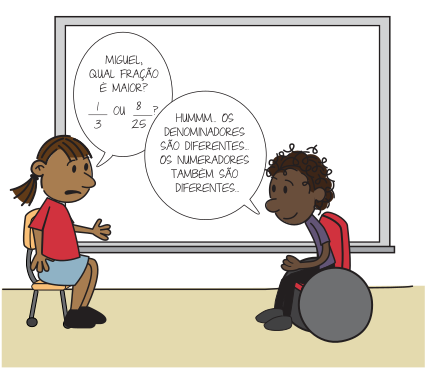
\includegraphics[width=.45\textwidth, keepaspectratio]{../../livro/media/cap4/secoes/PNGs/quadrinho_01.png} & 
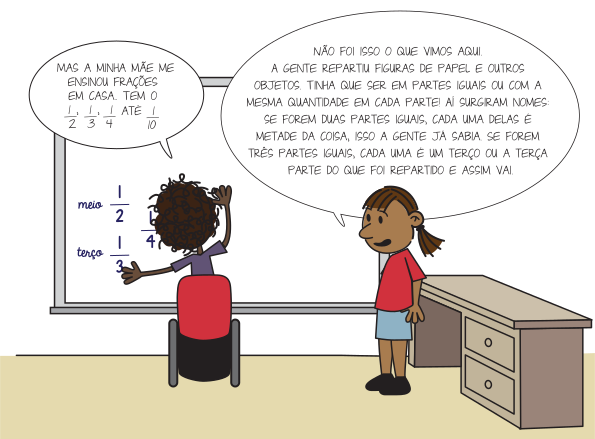
\includegraphics[width=.45\textwidth, keepaspectratio]{../../livro/media/cap4/secoes/PNGs/quadrinho_02.png} \\
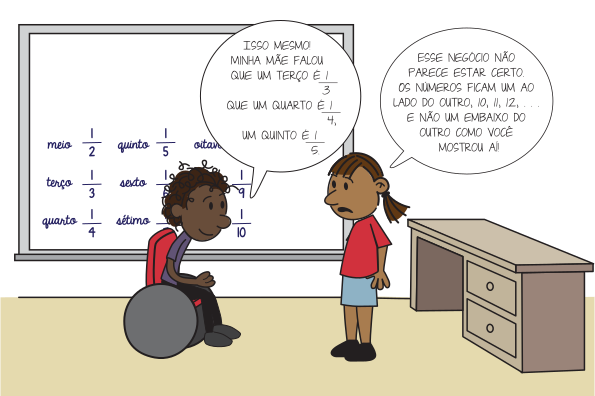
\includegraphics[width=.45\textwidth, keepaspectratio]{../../livro/media/cap4/secoes/PNGs/quadrinho_03.png} & 
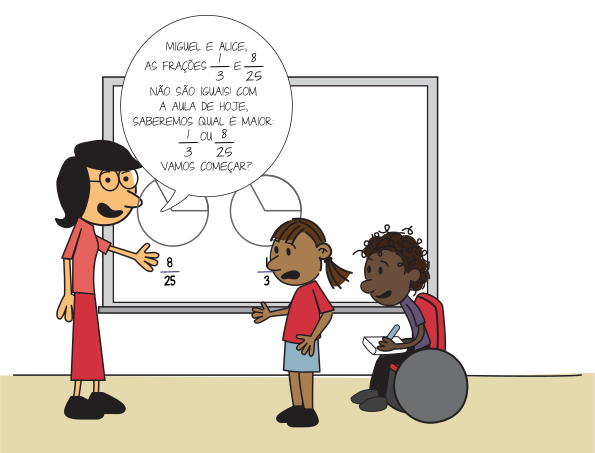
\includegraphics[width=.45\textwidth, keepaspectratio]{../../livro/media/cap4/secoes/PNGs/quadrinho_04.png}
         \end{tabular}

%\vspace*{-3cm}

\section{EXPLORANDO O ASSUNTO }

\subsection{Atividade}

A turma de Rita vai fazer um piquenique. A professora comprou pães para a turma preparar sanduíches. Cada colega preparou um sanduíche e partiu-o em partes iguais. Veja como alguns dos colegas repartiram o seu sanduiche: 


\begin{center}
\begin{tabular}{cccc}
\begin{tikzpicture}
\draw[fill=common, fill opacity=.3] (0,0) rectangle (20,20);
\draw (0,0) -- (20,20);
\node[below] at (10,0){(A)};
\end{tikzpicture}
&
\begin{tikzpicture}
\draw[fill=common, fill opacity=.3] (0,0) rectangle (20,20);
\draw (0,20/3) -- (20,20/3);
\draw (0,40/3) -- (20,40/3);
\node[below] at (10,0){(B)};
\end{tikzpicture}
&
\begin{tikzpicture}
\draw[fill=common, fill opacity=.3] (0,0) rectangle (20,20);
\draw (0,0) -- (20,20);
\draw (20,0) -- (0,20);
\node[below] at (10,0){(C)};
\end{tikzpicture}
&
\begin{tikzpicture}
\draw[fill=common, fill opacity=.3] (0,0) rectangle (20,20);
\draw (10,0) -- (10,20);
\draw (0,10) -- (20,10);
\node[below] at (10,0){(D)};
\end{tikzpicture}
\end{tabular}
\end{center}


\begin{enumerate} [\quad a)] %s
  \item     Nessas repartições, que fração do sanduíche pode representar cada uma das partes em que o sanduíche foi repartido?
  \item     Em quais dessas repartições é possível comer metade do sanduíche apenas com as partes em que o sanduíche foi repartido? Justifique sua resposta!
  \item     Para cada uma das repartições que você deu como resposta no Item (b), expresse, por meio de frações, a metade do sanduíche.
\end{enumerate} %s

\subsection{Atividade}

Junte-se a seus colegas e dobrem o retângulo da página de reprodução como indicado na coluna mais à esquerda da tabela. Observando as dobras feitas, responda às questões propostas, preenchendo a tabela. Divida o trabalho em sua equipe: cada membro pode ficar encarregado de uma ou mais linhas da tabela. Lembre-se: as dobraduras devem ser feitas perpendicularmente às várias linhas desenhadas no retângulo da página de reprodução.


  \begin{longtable}{|m{.30\textwidth}|m{.16\textwidth}|m{.16\textwidth}|m{.31\textwidth}|}
    \hline
      Como dobrar  &  Quantidade de retângulos pintados  & Quantidade total de retângulos  &  Fração do retângulo do encarte que está pintada  \\
    \hline \hline 
    \endhead
    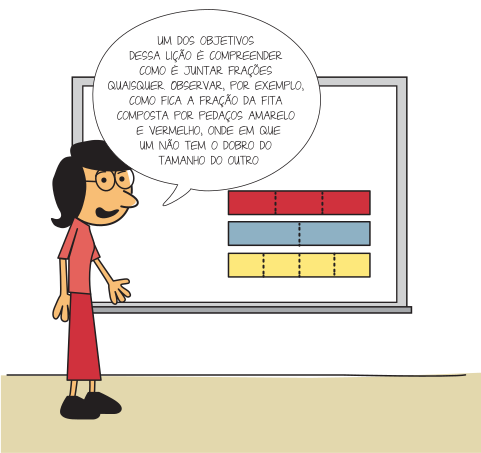
\includegraphics[width=110pt, keepaspectratio]{../../livro/media//cap4/secoes/PNGs/ativ2_fig01.png}      & $$3$$  & $$10$$   & $$\dfrac{3}{10}$$       \\
    \hline
     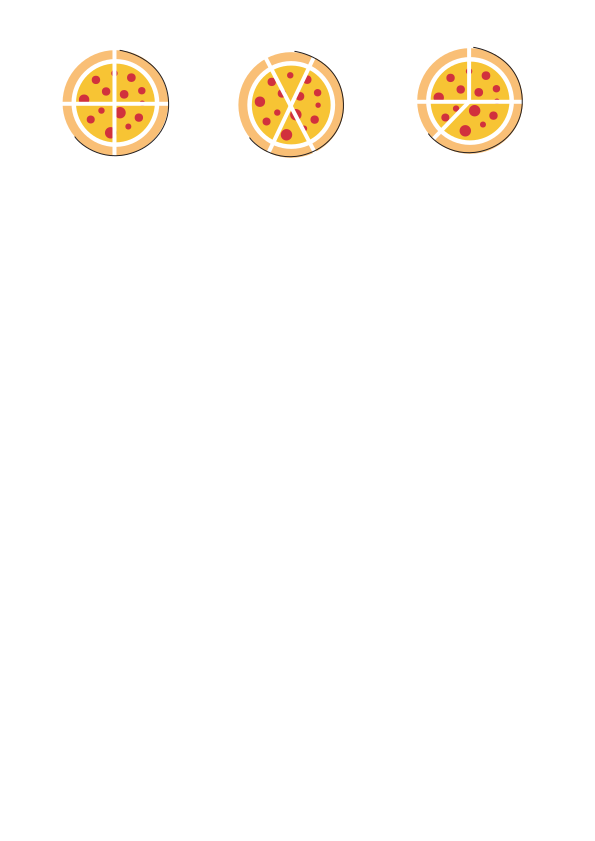
\includegraphics[width=110pt, keepaspectratio]{../../livro/media//cap4/secoes/PNGs/ativ2_fig02.png}                                                                              & &  &  \\
    \hline
     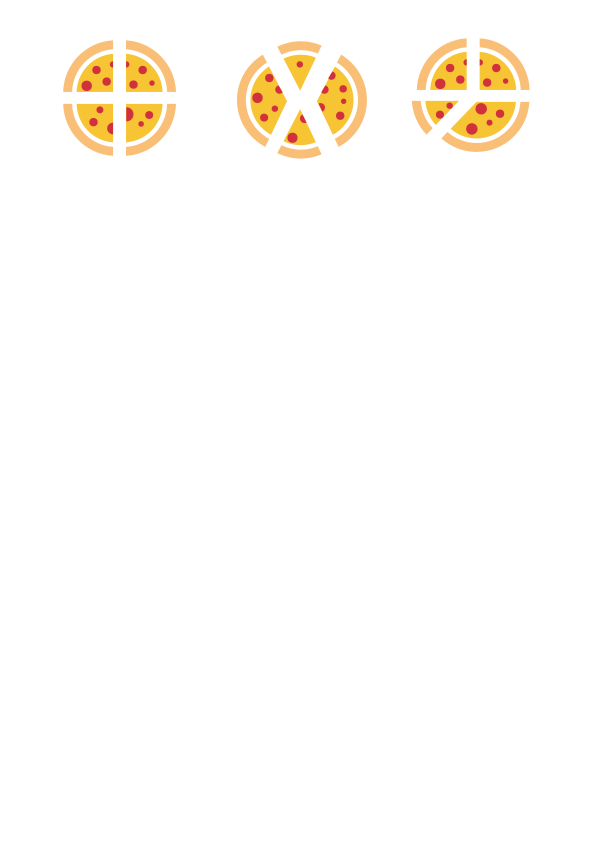
\includegraphics[width=110pt, keepaspectratio]{../../livro/media//cap4/secoes/PNGs/ativ2_fig03.png}     &  &   &  \\
    \hline
     \includegraphics[width=110pt, keepaspectratio]{../../livro/media//cap4/secoes/PNGs/ativ2_fig04.png} & &&\\
    \hline
     \includegraphics[width=110pt, keepaspectratio]{../../livro/media//cap4/secoes/PNGs/ativ2_fig05.png}  &                                     &                                  &                                                   \\
    \hline
     \includegraphics[width=110pt, keepaspectratio]{../../livro/media//cap4/secoes/PNGs/ativ2_fig06.png} &                                     &                                  &                                                   \\
    \hline
  \end{longtable}


\begin{refletindo*}

Na atividade 4 a folha foi divida inicialmente em dez retângulos iguais, dos quais três deles foram pintados de amarelo.

Ao realizar a primeira dobra, cada retângulo inicial ficou dividido ao meio, inclusive os pintados de amarelo. Assim, tanto para cobrir a área da região pintada de amarelo como para cobrir a área da folha será necessário o dobro da quantidade inicial:

Área da folha $=$ área de 10 retângulos $=$ área de 20 ``retângulos divididos ao meio'';\mbox{} \newline 
Área da região pintada $=$  área de 3 retângulos $=$ área de 6 ``retângulos divididos ao meio''.

Assim pode-se dizer que a área da região pintada de amarelo é $\frac{3}{10}$ ou  $\frac{6}{20}$ da área da folha. De onde se conclui que estas frações são iguais, pois elas representam a mesma quantidade: a área da região pintada de amarelo tendo a área da folha como unidade. Isto é,

$$\dfrac{3}{10} = \dfrac{6}{20} = \dfrac{2 \times 3}{2 \times 10},$$

onde 2 é o numero de partes em que você dobrou a folha.

Ora, quando você dobrou a folha em três partes iguais, cada retângulo inicial ficou dividido em três partes, inclusive os pintados de amarelo. Assim, tanto para cobrir a área da região pintada de amarelo como para cobrir a área da folha será necessário o triplo da quantidade inicial:

Área da folha $=$ área de 10 retângulos $=$ área de 30 ``retângulos divididos em três partes'';\mbox{} \newline 
Área da região pintada $=$  área de 3 retângulos $=$ área de 9 ``retângulos divididos em três partes''.

De onde se conclui que as frações $\frac{3}{10}$ e $\frac{9}{30}$  são iguais, pois elas representam a mesma quantidade: a área da região pintada de amarelo tendo a área da folha como unidade. Isto é,

$$\dfrac{3}{10} = \dfrac{9}{30} = \dfrac{3 \times 3}{3 \times 10},$$

onde 3 é o número de partes em que você dobrou a folha. 

Do mesmo modo, ao dobrar a folha em quatro, seis ou oito partes iguais, você obteve outras representações equivalentes para a fração $\frac{3}{10}$:
\begin{itemize} %d
  \item     ao dobrar em     {\bf quatro}     partes iguais:     $\frac{3}{10} = \frac{12}{40} = \frac{4 \times 3}{4 \times 10}$; em que 4 é o numero de partes em que você dobrou a folha;
  \item     ao dobrar em     {\bf seis}     partes iguais:     $\frac{3}{10} = \frac{18}{60} = \frac{6 \times 3}{6 \times 10}$; em que 6 é o numero de partes em que você dobrou a folha;
  \item     ao dobrar em     {\bf oito}     partes iguais:     $\frac{3}{10} = \frac{24}{80} = \frac{8 \times 3}{8 \times 10}$; em que 8 é o numero de partes em que você dobrou a folha.
\end{itemize} %d


Assim, generalizando o processo de ``dobrar'' a folha, tem-se que, ao ``dobrar'' a folha em $n$ partes iguais:

$$\dfrac{3}{10}=\dfrac{n \times 3}{n \times 10}\text{, onde n é o numero de partes em que você dobrou a folha.}$$

Agora, recomenda-se que você utilize o aplicativo disponível no link a seguir \url{http://tube.geogebra.org/m/X52U83TR} para dobrar a folha em partes cada vez menores (basta aumentar o valor de $m$ no aplicativo). Mexa à vontade! Qualquer dúvida pergunte ao seu professor.
\begin{center}
\includegraphics[width=300pt, keepaspectratio]{../../livro/media//cap4/secoes/dobradura-geogebra.png}
\end{center}
\end{refletindo*}


\subsection{Atividade}

(Garcez, 2013)

\begin{enumerate} [\quad a)] %s
  \item     O retângulo desenhado a seguir está dividido em     $4$     partes iguais, dais quais     $3$     estão pintadas de azul. Que fração do retângulo está pintada de azul?       
  \begin{center}
\begin{tikzpicture}[scale=.8]
\draw[fill=common] (0,0) rectangle (30,30);
\draw (30,0) rectangle (40,30);
\draw  (10,0)-- (10,30);
\draw  (20,0)-- (20,30);
\end{tikzpicture}
\end{center}

\item     O retângulo do item anterior foi dividido com o acréscimo de onze linhas horizontais igualmente espaçadas e ele está parcialmente coberto com um retângulo vermelho que impede a visualização dos retângulos menores que compõem a nova equipartição. Com essa nova divisão, em quantas partes fica dividido o retângulo? Quantas destas partes estão pintadas de azul? Que fração do retângulo está pintada de azul?     \mbox{} \newline      
\end{enumerate} %s

\begin{center}
\begin{tikzpicture}[scale=.8]
\draw[fill=common] (0,0) rectangle (30,30);
\draw (30,0) rectangle (40,30);
\draw  (10,0)-- (10,30);
\draw  (20,0)-- (20,30);
\foreach \x in {1,...,11}{
\draw (0,\x*30/12) -- (40,\x*30/12);}
\fill[attention] (5,-10) rectangle (55,29);
\end{tikzpicture}
\end{center}

\subsection{Atividade}
Rita convidou seus colegas de escola para virem à sua casa conhecer seu novo cãozinho. Sua mãe preparou um bolo para o lanche da tarde das crianças. Às 16h chegaram dois de seus colegas, João e Mário. Mário logo imaginou o bolo repartido em 3 pedaços e pensou que ele poderia então comer um terço do mesmo 

\begin{center}
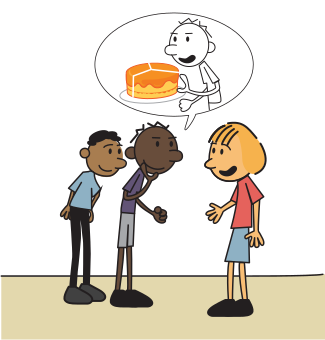
\includegraphics[width=.5\textwidth, keepaspectratio]{../../livro/media/cap4/secoes/PNGs/ativ4_fig01.png}
\end{center}

A mãe de Rita começou a cortar o bolo, partindo-o, como Mário havia imaginado, em 3 partes. No entanto, antes que começassem a comer, chegaram mais 4 colegas da escola. Então a mãe de Rita dividiu cada um dos 3 pedaços iniciais em 4 partes de igual tamanho 

\begin{center}
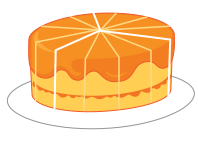
\includegraphics[width=.25\textwidth, keepaspectratio]{../../livro/media/cap4/secoes/PNGs/ativ4_fig02.png}
\end{center}



Na hora do lanche, João comeu 2 pedaços do bolo e Mário comeu 4.
\begin{itemize} %s
  \item     Que fração do bolo Mário comeu?
  \item     Que fração do bolo João comeu?
\end{itemize} %s

Se os amigos atrasados não tivessem aparecido antes do lanche, a mãe de Rita não teria divido as 3 fatias iniciais. Assim, se fossem apenas Rita, Mário e João, cada um teria comido uma das três fatias iniciais.
\begin{itemize} %s
  \item     Nesse caso, Mário teria comido menos bolo, mais bolo ou a mesma quantidade de bolo que comeu?
  \item     E João, teria comido menos bolo, mais bolo ou a mesma quantidade de bolo que comeu?
\end{itemize} %s


\subsection{Atividade}

O objetivo desta atividade é estudar a fração do círculo que está pintada de cinza no encarte que você recebeu.

\begin{center}
 
\begin{tikzpicture}
  \draw[fill=gray] (20,0) arc (0:240:20) -- (0,0)--cycle;
  \draw (0,0) circle (20);
 \end{tikzpicture}
\end{center}

Para isto, responda às perguntas na tabela a seguir com frações adequadas. Se necessário, use as peças coloridas que você recortou e usou na Atividade 10 da Lição 1 para avaliar as suas respostas. 

  \noindent \begin{longtable}{|m{0.25\textwidth}|m{0.2\textwidth}|m{0.2\textwidth}|m{0.2\textwidth}|}
    \hline
     Tipo da peça &   Quantas peças como essa cabem na região cinza? &   As peças que você usou, juntas, são que fração do círculo?  &  Que fração do círculo não está colorida de cinza? \\
    \hline \hline
    \endhead
     $\frac{1}{3}$ 
\begin{center}
 \begin{tikzpicture}[scale=.8]
  \draw[fill=common] (20,0) arc (0:120:20) -- (0,0)--cycle;
 \end{tikzpicture}
\end{center}
     &  &  &  \\
    \hline
     $\frac{1}{6}$ 
\begin{center}
\begin{tikzpicture}[scale=.8]
  \draw[fill=light] (20,0) arc (0:60:20) -- (0,0)--cycle;
\end{tikzpicture}
\end{center}
     &  &  &  \\
    \hline
     $\frac{1}{12}$ 
\begin{center}
\begin{tikzpicture}[scale=.8]
  \draw[fill=special] (20,0) arc (0:30:20) -- (0,0)--cycle;
\end{tikzpicture}
 \end{center}
&  &  &  \\
    \hline
  \end{longtable}


\begin{refletindo*}[breakable]{}{}     

Ao resolver esta última atividade você deve ter percebido que a região do círculo destacada em cinza pode ser preenchida de diferentes maneiras por justaposições de cada uma das peças coloridas que você recortou.    
\begin{center}
\begin{tabular}{b{.2\textwidth}b{.2\textwidth}b{.2\textwidth} b{.2\textwidth}}

\begin{center}
 
\begin{tikzpicture}
  \draw[fill=gray] (10,0) arc (0:240:10) -- (0,0)--cycle;
  \draw (0,0) circle (10);
 \end{tikzpicture}
\end{center}  
&
\begin{center}
 \begin{tikzpicture}
  \draw[fill=common] (10,0) arc (0:120:10) -- (0,0)--cycle;
 \end{tikzpicture}
\end{center}
&
\begin{center}
\begin{tikzpicture}
  \draw[fill=light] (10,0) arc (0:60:10) -- (0,0)--cycle;
\end{tikzpicture}
\end{center}
&
\begin{center}
\begin{tikzpicture}
  \draw[fill=special] (10,0) arc (0:30:10) -- (0,0)--cycle;
\end{tikzpicture}
\end{center}
\end{tabular}
\end{center}

Além disso, deve ter observado que, quanto menor a peça colorida, mais dessas peças você precisou para cobrir a região do círculo destacada em cinza.  
  
Ao preencher a   {\bf primeira linha da tabela}, você deve ter percebido que três peças azuis cobrem o círculo inteiro e que duas peças azuis cobrem a região do círculo destacada em cinza.  
  
\begin{tabular}{m{.45\textwidth}m{.45\textwidth}}
\begin{center}
 \begin{tikzpicture}
  \draw[fill=common] (10,0) arc (0:120:10) -- (0,0)--cycle;
  \draw[fill=common] (120:10) arc (120:240:10) -- (0,0)--cycle;
  \draw[fill=common] (240:10) arc (240:360:10) -- (0,0)--cycle;
 \end{tikzpicture}
\end{center}
&
\begin{center}
 \begin{tikzpicture}
  \draw[fill=common] (10,0) arc (0:120:10) -- (0,0)--cycle;
  \draw[fill=common] (120:10) arc (120:240:10) -- (0,0)--cycle;
  \draw (0,0) circle (10);
\end{tikzpicture}
\end{center}
\end{tabular}

Portanto, a região do círculo destacada em cinza é igual a   $\frac{2}{3}$   do círculo.  
  
  Para preencher a   {\bf segunda linha da tabela}   você deve ter percebido que   
\begin{itemize} %s
    \item       que seis peças laranjas cobrem o círculo inteiro; 
\end{itemize} %s
  
\begin{tabular}{m{.45\textwidth}m{.45\textwidth}}
\begin{center}
\begin{tikzpicture}
  \draw[fill=light] (0,0) circle (10);
  \foreach \x in {0,60,...,360} \draw (0,0) -- (\x:10);
\end{tikzpicture}
\end{center}
&
\begin{center}
\begin{tikzpicture}
  \draw[fill=light] (10,0) arc (0:60:10) -- (0,0)--cycle;
  \foreach \x in {0,60,...,360} \draw (0,0) -- (\x:10);
  \draw (0,0) circle (10);
\end{tikzpicture}
\end{center}
\end{tabular}

\begin{itemize} %s
    \item       que duas peças laranjas cobrem uma peça azul; 
\end{itemize} %s

\begin{tabular}{m{.45\textwidth}m{.45\textwidth}}
\begin{center}
 \begin{tikzpicture}
  \draw[fill=common] (10,0) arc (0:120:10) -- (0,0)--cycle;
  \draw (0,0) circle (10);
  \draw (0,0) -- (240:10);
 \end{tikzpicture}
\end{center}
&
\begin{center}
\begin{tikzpicture}
  \draw[fill=light] (10,0) arc (0:120:10) -- (0,0)--cycle;
  \foreach \x in {0,60,...,360} \draw (0,0) -- (\x:10);
  \draw (0,0) circle (10);
\end{tikzpicture}
\end{center}
\end{tabular}

\begin{itemize} %s
    \item       e que quatro peças laranjas cobrem a região do círculo destacada em cinza. 
\end{itemize} %s
  
  \begin{tabular}{m{.45\textwidth}m{.45\textwidth}}
\begin{center}
 \begin{tikzpicture}
  \draw[fill=common] (10,0) arc (0:120:10) -- (0,0)--cycle;
  \draw[fill=common] (120:10) arc (120:240:10) -- (0,0)--cycle;
  \draw (0,0) circle (10);
\end{tikzpicture}
\end{center}
&
\begin{center}
\begin{tikzpicture}
  \draw[fill=light] (10,0) arc (0:240:10) -- (0,0)--cycle;
  \foreach \x in {0,60,...,360} \draw (0,0) -- (\x:10);
  \draw (0,0) circle (10);
\end{tikzpicture}
\end{center}
  \end{tabular}

  $\left(\frac{4}{6} = \frac{2\times 2}{2\times 3} = \frac{2}{3} \right)$  
  Portanto, a região do círculo destacada em cinza é igual a   $\frac{4}{6}$   do círculo.  
  
  Este raciocínio pode ser escrito da seguinte maneira:  
  $\frac{1}{3}$   é igual a dois   $\frac{1}{6}$  , ou, simplesmente,   
  $\frac{1}{3}   =   \frac{2}{6}$  .  

\begin{tabular}{m{.45\textwidth}m{.45\textwidth}}
\begin{center}
 \begin{tikzpicture}
  \draw[fill=common] (10,0) arc (0:120:10) -- (0,0)--cycle;
  \draw (0,0) circle (10);
  \draw (0,0) -- (240:10);
 \end{tikzpicture}
\end{center}
&
\begin{center}
\begin{tikzpicture}
  \draw[fill=light] (10,0) arc (0:120:10) -- (0,0)--cycle;
  \foreach \x in {0,60,...,360} \draw (0,0) -- (\x:10);
  \draw (0,0) circle (10);
\end{tikzpicture}
\end{center}
\end{tabular}

  Logo,  $\frac{4}{6} = \frac{2 \times 2}{2 \times 3} = \frac{2}{3}$  .  

\begin{tabular}{m{.45\textwidth}m{.45\textwidth}}
\begin{center}
 \begin{tikzpicture}
  \draw[fill=common] (10,0) arc (0:120:10) -- (0,0)--cycle;
  \draw[fill=common] (120:10) arc (120:240:10) -- (0,0)--cycle;
  \draw (0,0) circle (10);
\end{tikzpicture}
\end{center}
&
\begin{center}
\begin{tikzpicture}
  \draw[fill=light] (10,0) arc (0:240:10) -- (0,0)--cycle;
  \foreach \x in {0,60,...,360} \draw (0,0) -- (\x:10);
  \draw (0,0) circle (10);
\end{tikzpicture}
\end{center}
  \end{tabular}
  
  Do mesmo modo, para preencher a   {\bf terceira linha da tabela}   você deve ter percebido:  
\begin{itemize} %d
    \item       que doze peças vermelhas cobrem o círculo inteiro; 
\end{itemize} %d

\begin{center}
  \begin{tikzpicture}
  \draw[fill=special] (0,0) circle (10);
  \foreach \x in {0,30,...,360} \draw (0,0) -- (\x:10);
\end{tikzpicture}
\end{center}

\begin{itemize} %d
    \item       que quatro peças vermelhas cobrem uma peça azul; 
\end{itemize} %d
\begin{tabular}{m{.45\textwidth}m{.45\textwidth}}
\begin{center}
 \begin{tikzpicture}
  \draw[fill=common] (10,0) arc (0:120:10) -- (0,0)--cycle;
  \draw (0,0) circle (10);
  \draw (0,0) -- (240:10);
\end{tikzpicture}
\end{center}
&
\begin{center}
  \begin{tikzpicture}
  \draw[fill=special] (0,0) -- (10,0) arc (0:120:10) -- cycle;
  \foreach \x in {0,30,...,360} \draw (0,0) -- (\x:10);
  \draw (0,0) circle (10);
\end{tikzpicture}
\end{center}
\end{tabular}
\begin{itemize} %d
    \item       e que oito peças vermelhas cobrem a região do círculo destacada em cinza. 
\end{itemize} %d
  
\begin{tabular}{m{.45\textwidth}m{.45\textwidth}}
\begin{center}
 \begin{tikzpicture}
  \draw[fill=common] (10,0) arc (0:120:10) -- (0,0)--cycle;
  \draw[fill=common] (120:10) arc (120:240:10) -- (0,0)--cycle;
  \draw (0,0) circle (10);
\end{tikzpicture}
\end{center}
&
\begin{center}
\begin{tikzpicture}
  \draw[fill=special] (10,0) arc (0:240:10) -- (0,0)--cycle;
  \foreach \x in {0,30,...,360} \draw (0,0) -- (\x:10);
  \draw (0,0) circle (10);
\end{tikzpicture}
\end{center}
  \end{tabular}
  
  $$\left(\frac{8}{12} = \frac{4\times 2}{4\times 3} = \frac{2}{3} \right)$$
  
  Logo, a região do círculo destacada em cinza é igual a   $\frac{8}{12}$   do círculo.   
  
  Este raciocínio pode ser representado do seguinte modo:  
  $\frac{1}{3}$   é igual a quatro   $\frac{1}{12}$  , ou, simplesmente,   
  $\frac{1}{3}=\frac{4}{12}$  

  \begin{tabular}{m{.45\textwidth}m{.45\textwidth}}
\begin{center}
 \begin{tikzpicture}
  \draw[fill=common] (10,0) arc (0:120:10) -- (0,0)--cycle;
  \draw (0,0) circle (10);
  \draw (0,0) -- (240:10);
\end{tikzpicture}
\end{center}
&
\begin{center}
  \begin{tikzpicture}
  \draw[fill=special] (0,0) -- (10,0) arc (0:120:10) -- cycle;
  \foreach \x in {0,30,...,360} \draw (0,0) -- (\x:10);
  \draw (0,0) circle (10);
\end{tikzpicture}
\end{center}
\end{tabular}

Logo,  
  $$\dfrac{8}{12} = \dfrac{4\times 2}{4 \times 3} = \dfrac{2}{3}.$$  
  
\begin{tabular}{m{.45\textwidth}m{.45\textwidth}}
\begin{center}
 \begin{tikzpicture}
  \draw[fill=common] (10,0) arc (0:120:10) -- (0,0)--cycle;
  \draw[fill=common] (120:10) arc (120:240:10) -- (0,0)--cycle;
  \draw (0,0) circle (10);
\end{tikzpicture}
\end{center}
&
\begin{center}
\begin{tikzpicture}
  \draw[fill=special] (10,0) arc (0:240:10) -- (0,0)--cycle;
  \foreach \x in {0,30,...,360} \draw (0,0) -- (\x:10);
  \draw (0,0) circle (10);
\end{tikzpicture}
\end{center}
  \end{tabular}
  Portanto, a região do círculo destacada em cinza, que é   $\frac{2}{3}$   do círculo, também é igual a   $\frac{4}{6}$   do círculo e igual a   $\frac{8}{12}$   do círculo, ou seja, as frações    $\frac{2}{3}$  ,   $\frac{4}{6}$    e   $\frac{8}{12}$   representam a mesma quantidade e, portanto, são iguais:  
  $$\frac{2}{3}   =   \frac{4}{6}   =   \frac{8}{12}.$$  
  
\end{refletindo*}


\subsection{Atividade}

{\bf PARTE 1}

Você recebeu um encarte com 10 retângulos coloridos de mesmo tamanho, cada deles dividido em um determinado número de partes iguais. Seguindo o modelo feito para o primeiro retângulo, preencha a tabela a seguir.


\begin{center}
  \begin{longtable}{|m{.4\textwidth}|m{.25\textwidth}|m{.25\textwidth}|}
    \hline
      \centering Retângulo  &   Número de partes em se encontra dividido  &   Cada parte é que fração do retângulo?  \\
    \hline \hline
    \endhead
   \centering 
    \begin{tikzpicture}
\draw[fill=light] (0,0) rectangle (60,12);
\draw (30,0) -- (30,12);
    \end{tikzpicture}   &   \centering $2$  & \parbox[t][1.3 cm][c]{.25\textwidth}{ \centering $\dfrac{1}{2}$ } \\
    \hline
 \centering  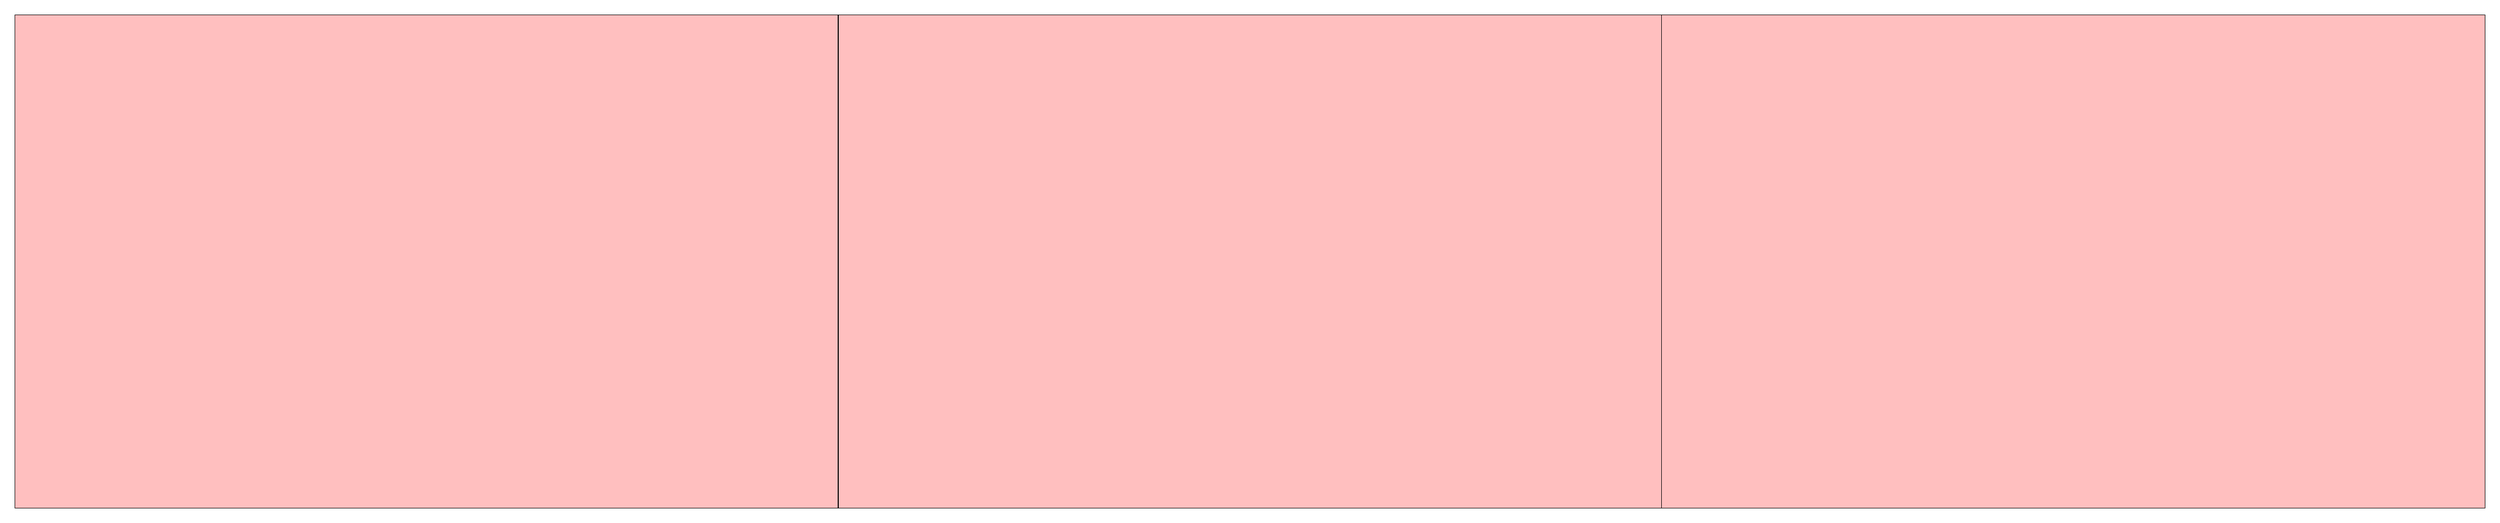
\begin{tikzpicture}
\draw[fill=pink] (0,0) rectangle (60,12);
\foreach \x in {1,2} \draw (\x*60/3,0) -- (\x*60/3,12);
    \end{tikzpicture}        &  \parbox[t][1.3 cm][c]{.2cm}{ }    &     \\
    \hline
    \centering  \begin{tikzpicture}
\draw[fill=special] (0,0) rectangle (60,12);
\foreach \x in {1,2,3} \draw (\x*60/4,0) -- (\x*60/4,12);
    \end{tikzpicture}        &  \parbox[t][1.3 cm][c]{.2cm}{ }    &     \\
    \hline
 \centering  \begin{tikzpicture}
\draw[fill=attention] (0,0) rectangle (60,12);
\foreach \x in {1,...,4} \draw (\x*60/5,0) -- (\x*60/5,12);
    \end{tikzpicture}        &  \parbox[t][1.3 cm][c]{.2cm}{ }    &     \\
    \hline
 \centering  \begin{tikzpicture}
\draw[fill=common] (0,0) rectangle (60,12);
\foreach \x in {1,...,5} \draw (\x*60/6,0) -- (\x*60/6,12);
    \end{tikzpicture}        &  \parbox[t][1.3 cm][c]{.2cm}{ }    &     \\
    \hline
  \centering  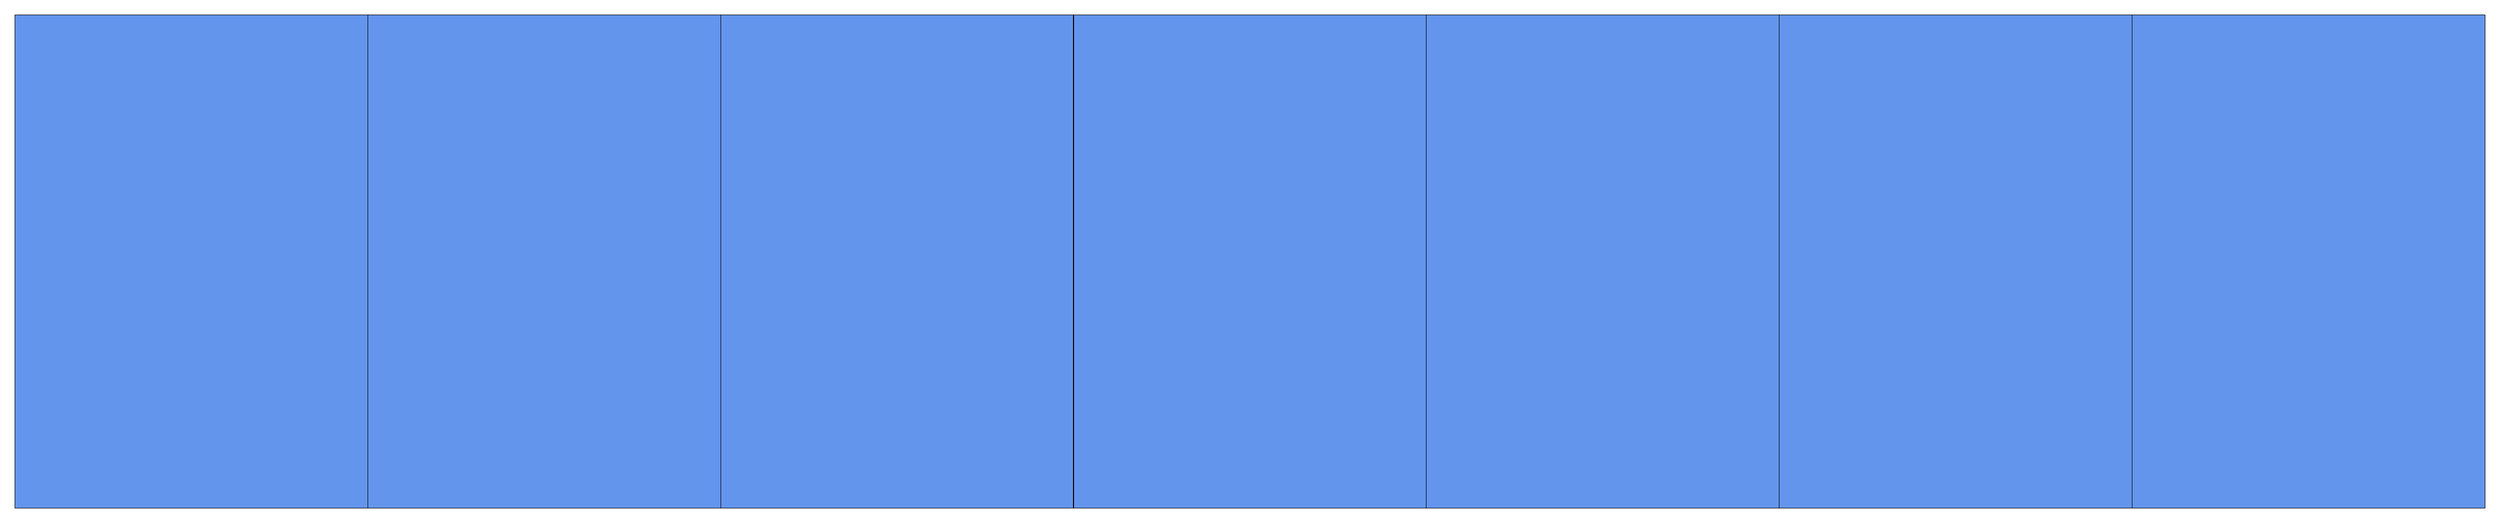
\begin{tikzpicture}
\draw[fill=CornflowerBlue] (0,0) rectangle (60,12);
\foreach \x in {1,...,6} \draw (\x*60/7,0) -- (\x*60/7,12);
    \end{tikzpicture}        &  \parbox[t][1.3 cm][c]{.2cm}{ }    &     \\
    \hline
 \centering  \begin{tikzpicture}
\draw[fill=dark] (0,0) rectangle (60,12);
\foreach \x in {1,...,7} \draw (\x*60/8,0) -- (\x*60/8,12);
    \end{tikzpicture}        &  \parbox[t][1.3 cm][c]{.2cm}{ }    &     \\
    \hline
 \centering  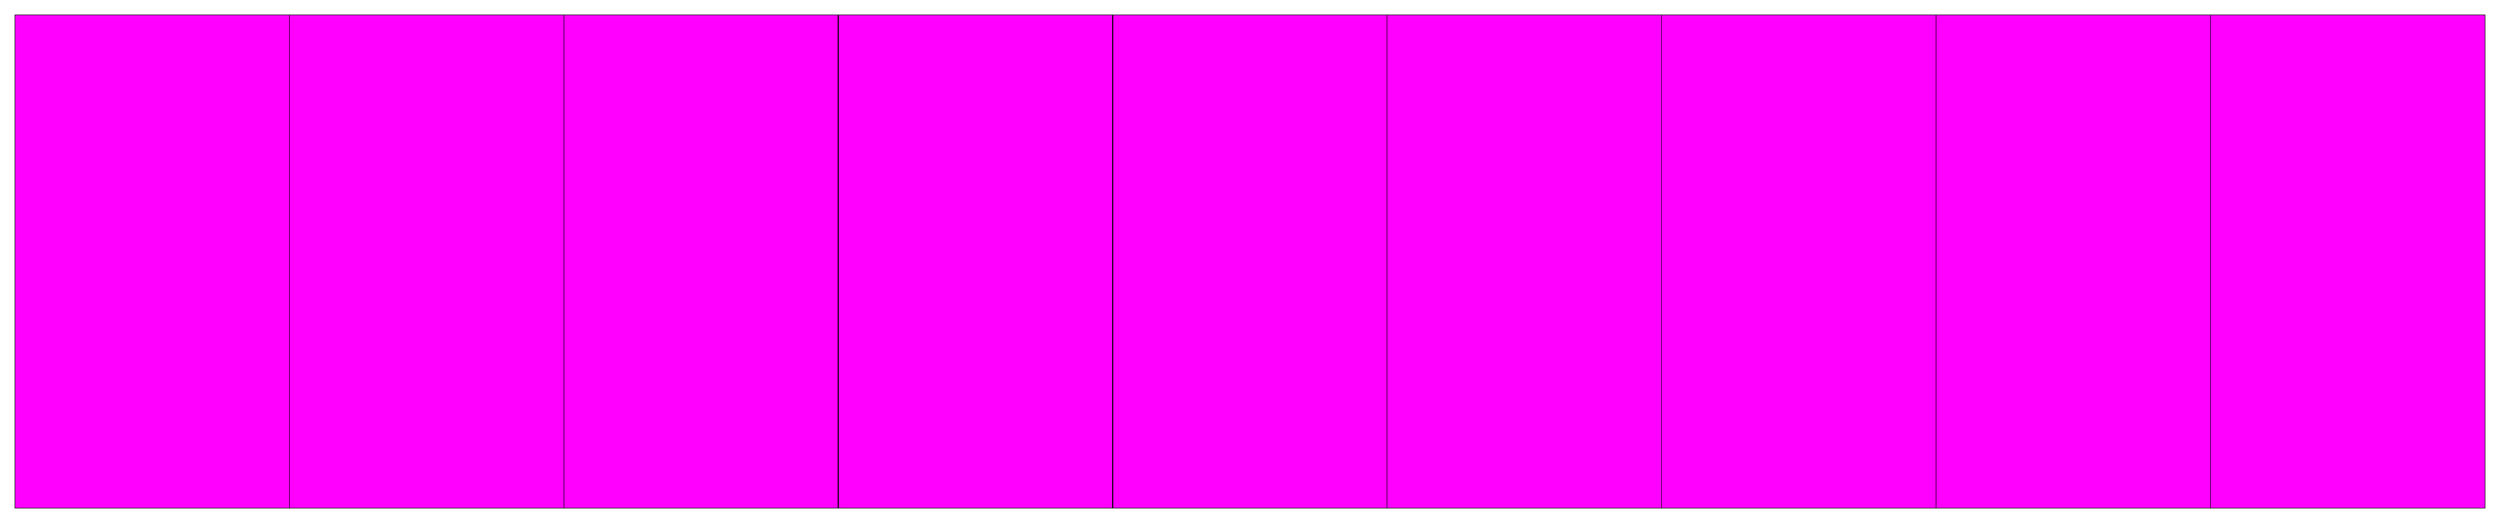
\begin{tikzpicture}
\draw[fill=Fuchsia] (0,0) rectangle (60,12);
\foreach \x in {1,...,8} \draw (\x*60/9,0) -- (\x*60/9,12);
    \end{tikzpicture}        &  \parbox[t][1.3 cm][c]{.2cm}{ }    &     \\
    \hline
 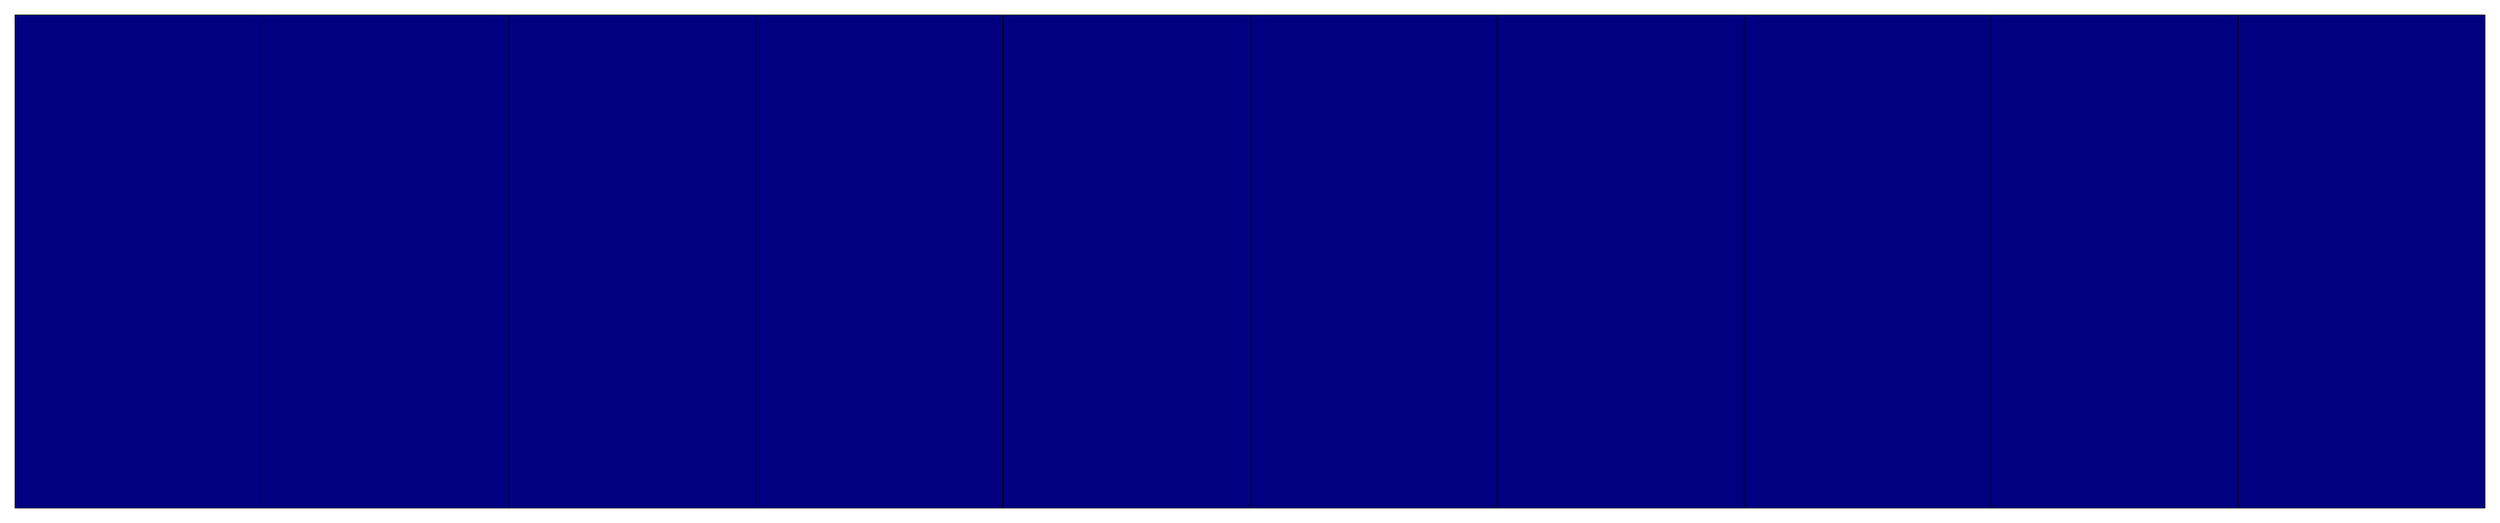
\begin{tikzpicture}   
 \draw[fill=NavyBlue] (0,0) rectangle (60,12);
 \foreach \x in {1,...,9} \draw (\x*60/10,0) -- (\x*60/10,12);
     \end{tikzpicture}        &  \parbox[t][1.3 cm][c]{.2cm}{ }    &     \\
    \hline
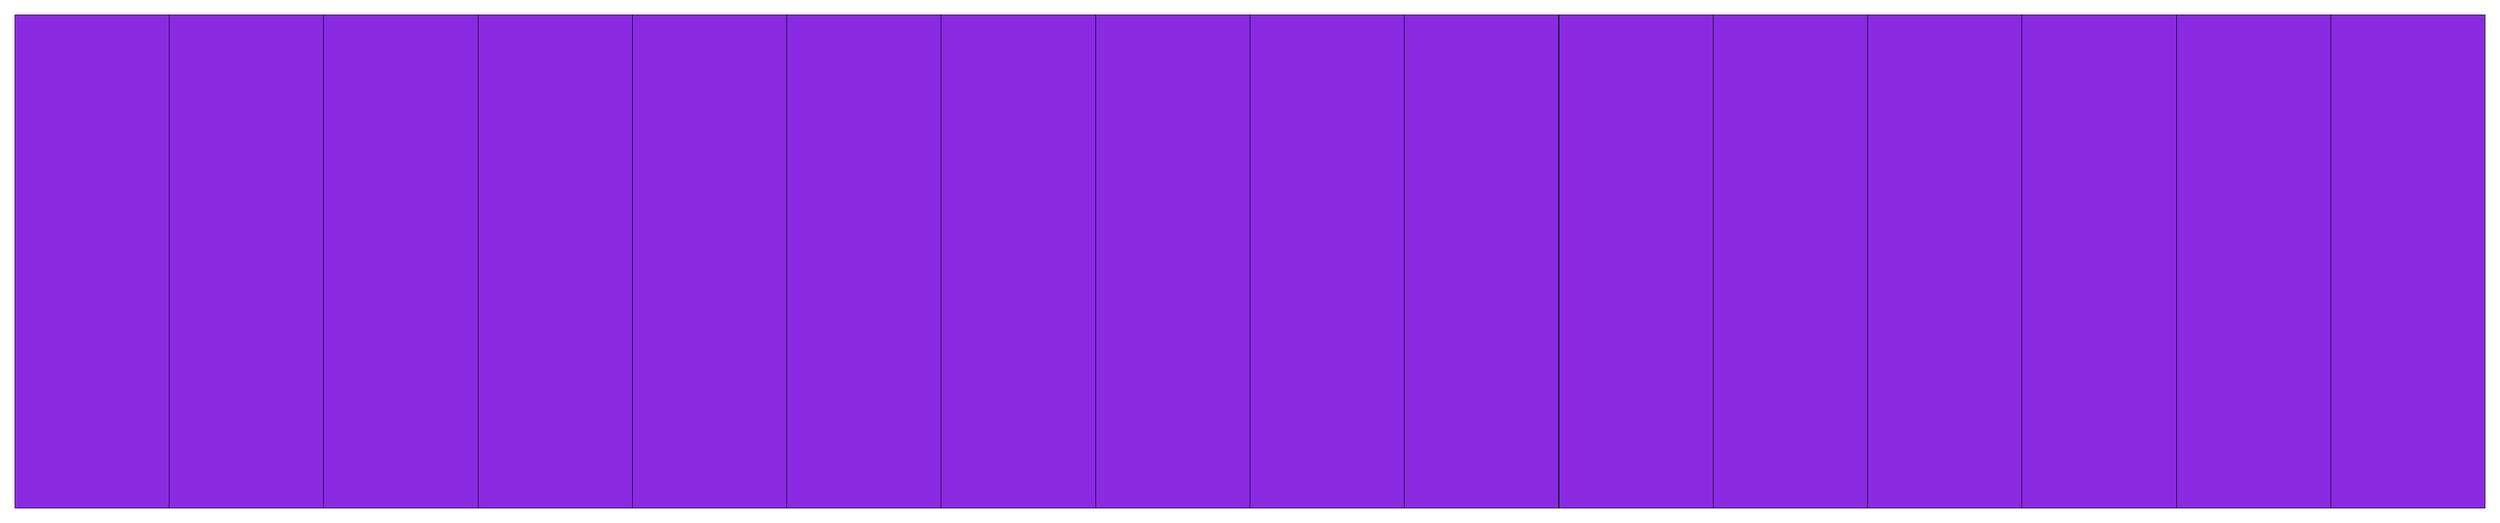
\begin{tikzpicture}   
    \draw[fill=BlueViolet] (0,0) rectangle (60,12);
\foreach \x in {1,...,15} \draw (\x*60/16,0) -- (\x*60/16,12);
    \end{tikzpicture}        &  \parbox[t][1.3 cm][c]{.2cm}{ }    &     \\
    \hline 
 \end{longtable}
\end{center}

{\bf PARTE 2}

O objetivo desta parte é estudar a fração do retângulo que está colorida de cinza no segundo encarte que você recebeu. 
\begin{center}
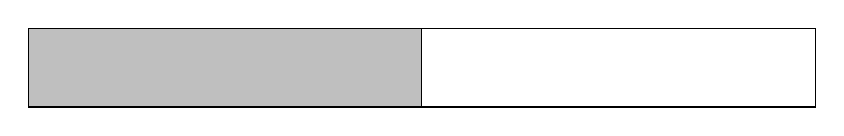
\begin{tikzpicture}[x=1mm, y=1mm]
% Fita principal (metade cinza, metade branca)
\draw (0,0) rectangle (100,10);
\draw[fill=lightgray] (0,0) rectangle (100/2,10);
\end{tikzpicture}
\end{center}

Para isto, responda às perguntas na tabela a seguir com frações adequadas. Se necessário, recorte e use as peças coloridas do primeiro encarte para avaliar as suas respostas.

\begin{center}
  \begin{longtable}{|m{.35\textwidth}|m{.16\textwidth}|m{.18\textwidth}|m{.19\textwidth}|}
 \hline
 \centering Tipo da peça &   Quantas peças como essa cabem na região cinza? &   As peças que você usou, juntas, são que fração do retângulo do encarte?  &  Que fração do retângulo do encarte não está colorida de cinza? \\
    \hline    \hline
\centering \begin{tikzpicture}[x=1mm, y=1mm]
% Fita de largura 1/2
\draw[fill=light] (0,0) rectangle (100/2,10);
\end{tikzpicture} &  \parbox[t][1.3 cm][c]{.2cm}{ } &  &  \\
    \hline
\centering  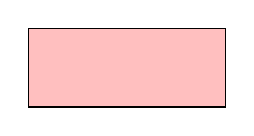
\begin{tikzpicture}[x=1mm, y=1mm]
% Fita rosa de largura 1/4
\draw[fill=pink] (0,0) rectangle (100/4,10);
\end{tikzpicture}
        &  \parbox[t][1.3 cm][c]{.2cm}{ } &  &  \\
    \hline
 \centering \begin{tikzpicture}[x=1mm, y=1mm]
% Fita rosa de largura 1/6
\draw[fill=special] (0,0) rectangle (100/6,10);
\end{tikzpicture}    &  \parbox[t][1.3 cm][c]{.2cm}{ } &  &  \\
    \hline
\centering \begin{tikzpicture}[x=1mm, y=1mm]
% Fita rosa de largura 1/8
\draw[fill=attention] (0,0) rectangle (100/8,10);
\end{tikzpicture}     &  \parbox[t][1.3 cm][c]{.2cm}{ } &  &  \\
    \hline
\centering \begin{tikzpicture}[x=1mm, y=1mm]
% Fita rosa de largura 1/10
\draw[fill=common] (0,0) rectangle (100/10,10);
\end{tikzpicture}     &  \parbox[t][1.3 cm][c]{.2cm}{ } &  &  \\
    \hline
\centering \begin{tikzpicture}[x=1mm, y=1mm]
% Fita rosa de largura 1/16
\draw[fill=CornflowerBlue] (0,0) rectangle (100/16,10);
\end{tikzpicture}     &  \parbox[t][1.3 cm][c]{.2cm}{ } &  &  \\
    \hline
  \end{longtable}
\end{center}

\begin{refletindo*}[breakable]{}{}  
  Você deve ter observado que as atividades 2 e 3 são muito parecidas.   
  A diferença é que, nesta última foram utilizadas figuras retangulares (na atividade 2 foram usadas figuras circulares).   
  Ao resolver esta atividade você deve ter percebido que   
  $$\dfrac{1}{2}=\dfrac{2}{4}=\dfrac{3}{6}=\dfrac{4}{8}=\dfrac{5}{10}=\dfrac{8}{16},$$  
  pois todas as frações representam a mesma quantidade: a medida da área da região retangular cinza em relação a área do retângulo do encarte.  
  Observe ainda que as igualdades acima podem ser reescritas do seguinte modo:  
  $$\dfrac{1}{2}=\dfrac{1 \times 1}{1 \times 2}= \dfrac{2 \times 1}{2 \times 2} =\dfrac{3 \times 1}{3 \times 2} = \dfrac{4 \times 1}{4 \times 2} = \dfrac{5 \times 1}{5 \times 2}= \dfrac{8 \times 1}{8 \times 2}.$$  
  Na verdade, para qualquer subdivisão da fração   $\frac{1}{2}$    em   $p$   partes iguais, deve-se considerar   $p$   dessas novas partes para obter uma fração igual a anterior. Matematicamente falando, isto significa que:  
  $$\dfrac{1}{2}= \dfrac{p \times 1}{p \times 2}$$     
  qualquer que seja   $p$   um número natural maior que zero.  
  De modo geral, para qualquer fração    $\frac{n}{d}$,  temos que  
  $$\dfrac{n}{d}=\dfrac{1 \times n}{1 \times d}= \dfrac{2 \times n}{2 \times d} = \dfrac{3 \times n}{3 \times d} = \dfrac{4 \times n}{4 \times d} = \dfrac{5 \times n}{5 \times d}=\cdots =  \dfrac{p \times n}{p \times d}= \cdots$$  
  qualquer que seja o número natural   $p > 0$.  
  Com isso, você aprendeu uma técnica para obter frações iguais a uma fração dada: basta multiplicar o numerador e o denominador da fração dada por um mesmo número natural   $p > 0$.   
  
  Isto será muito útil para a realização de outras atividades com frações.  
\end{refletindo*}



\subsection{Atividade}


\begin{enumerate} [\quad a)] %d
  \item     Preencha os quadradinhos     $\square$     com numeradores adequados de modo que cada fração corresponda a sua respectiva marca em cada reta numérica.    \mbox{} \newline      

 \begin{center}
 \begin{tikzpicture}[x=45mm,y=45mm]
  \draw (0,0) -- (3,0);
  \foreach \x in {0,...,3}{ 
  \draw (\x,-3pt) -- (\x, 3pt);
  \node[above] at (\x,3pt) {\x};}
  
  \foreach \x in {0,.333,...,3}{ 
  \draw (\x,-2pt) -- (\x, 2pt);
  \node[below] at (\x,-2 pt) {$\dfrac{\square}{3}$};
  \draw[dotted] (\x,-30pt) -- (\x, -60pt);
  }
  
  \fill[common] (1+1/3,0) circle (2pt);
  
  \begin{scope}[shift={(0,-75pt)}]
  \draw (0,0) -- (3,0);
  \foreach \x in {0,...,3}{ 
  \draw (\x,-3pt) -- (\x, 3pt);
  \node[above] at (\x,3pt) {\x};}
  
  \foreach \x in {0,.333,...,3}{ 
  \draw (\x,-2pt) -- (\x, 2pt);
  \node[below] at (\x,-2 pt) {$\dfrac{\square}{6}$};
  \draw[dotted] (\x,-30pt) -- (\x, -60pt);
  }
  
  \foreach \x in {0,.333,...,6}{ 
  \draw (\x/2,-2pt) -- (\x/2, 2pt);}
  
  
  \fill[common] (1+1/3,0) circle (2pt);
   
  \end{scope}

  
  \begin{scope}[shift={(0,-150pt)}]
  \draw (0,0) -- (3,0);
  \foreach \x in {0,...,3}{ 
  \draw (\x,-3pt) -- (\x, 3pt);
  \node[above] at (\x,3pt) {\x};}
  
  \foreach \x in {0,.333,...,3}{ 
  \draw (\x,-2pt) -- (\x, 2pt);
  \node[below] at (\x,-2 pt) {$\dfrac{\square}{9}$};
  \draw[dotted] (\x,-30pt) -- (\x, -60pt);
  }
  
  \foreach \x in {0,.333,...,9}{ 
  \draw (\x/3,-2pt) -- (\x/3, 2pt);}
  
  
  
  \fill[common] (1+1/3,0) circle (2pt);
   
  \end{scope}

  \begin{scope}[shift={(0,-225pt)}]
  \draw (0,0) -- (3,0);
  \foreach \x in {0,...,3}{ 
  \draw (\x,-3pt) -- (\x, 3pt);
  \node[above] at (\x,3pt) {\x};}
  
  \foreach \x in {0,.333,...,3}{ 
  \draw (\x,-2pt) -- (\x, 2pt);
  \node[below] at (\x,-2 pt) {$\dfrac{\square}{12}$};
  %\draw[dotted] (\x,-30pt) -- (\x, -60pt);
  }
  
  \foreach \x in {0,.333,...,12}{ 
  \draw (\x/4,-2pt) -- (\x/4, 2pt);}
  
  \fill[common] (1+1/3,0) circle (2pt);
   
  \end{scope} 
 \end{tikzpicture}
\end{center}
  \item     Escreva quatro frações com numeradores e denominadores diferentes que correspondam ao ponto azul em destaque na figura.
  \item     Determine uma fração de denominador     $15$     que corresponda ao ponto azul em destaque. Justifique sua resposta usando uma reta numérica!
\end{enumerate} %d

\begin{refletindo*}
Na Atividade 7, foram apresentadas quatro figuras que mostravam a reta numérica com subdivisões em partes iguais, mas de formas diferentes.

Na primeira figura, as subdivisões do segmento unitário (que está, aqui, servindo como unidade) eram em três partes iguais, ou seja, em terços. Para representar o ponto azul na reta numérica da primeira figura, foram consideradas quatro cópias de $\frac{1}{3}$, justapostas a partir da origem. Portanto, o ponto azul indica na reta numérica a fração $\frac{4}{3}$.
\begin{center}
\begin{tikzpicture}[x=45mm,y=45mm]
  \draw (0,0) -- (3,0);
  \foreach \x in {0,...,3}{ 
  \draw (\x,-3pt) -- (\x, 3pt);
  \node[above] at (\x,3pt) {\x};}

\fill[light] (1.3,-3pt) rectangle (1.37,-18pt);
  
  \foreach \x in {0,...,9}{ 
  \draw (\x/3,-2pt) -- (\x/3, 2pt);
  \node[below] at (\x/3,-2 pt) {$\dfrac{\x}{3}$};
  %\draw[dotted] (\x,-30pt) -- (\x, -60pt);
  }
  
  \fill[common] (1+1/3,0) circle (2pt);
\end{tikzpicture}
\end{center}

Na segunda figura, cada uma das subdivisões do segmento unitário foram divididas em duas partes iguais. Assim, as justaposições dos segmentos unitários ficam subdivididos em seis partes iguais, ou seja, em sextos. Para representar o ponto azul na reta numérica da segunda figura, foram necessárias então oito (o dobro da quantidade anterior) cópias de  $\frac{1}{6}$. Logo, o ponto azul representa também a fração $\frac{8}{6}$.

\begin{center}
\begin{tikzpicture}[x=45mm,y=45mm]
 \draw (0,0) -- (3,0);
  \foreach \x in {1,...,3}{ 
  \draw (\x,-3pt) -- (\x, 3pt);
  \node[above] at (\x,3pt) {\x};}
  
\fill[light] (1.3,-3pt) rectangle (1.37,-18pt);  
  
\foreach \x in {0,2,...,18}{ 
\draw (\x/6,-2pt) -- (\x/6, 2pt);
\node[below] at (\x/6,-2 pt) {$\dfrac{\x}{6}$};}
  
\foreach \x in {0,.333,...,6}{ 
\draw (\x/2,-2pt) -- (\x/2, 2pt);}
  
\fill[common] (1+1/3,0) circle (2pt);

\begin{scope}[shift={(0,.15)}]
 \draw[thick, |-|] (0,0) -- (1/3,0);
  \node[above] at (.33/2,0) {$\dfrac{1}{3}$};
  \draw[dotted] (0,-6pt) -- (0,-12pt);
  \draw[dotted] (.333,-6pt) -- (.333,-12pt);
  \end{scope}

\end{tikzpicture}
\end{center}


Isto é,
$$\dfrac{4}{3} = \dfrac{2 \times 4}{2 \times 3} = \dfrac{8}{6}.$$

Na terceira figura, cada uma das três subdivisões do segmento unitário apresentadas na primeira figura foi dividida em três partes iguais. Assim, as justaposições dos segmentos unitários ficam subdivididos em nove partes iguais, ou seja, em nonos. Para representar o ponto azul na reta numérica da terceira figura, foram necessárias doze (o triplo da quantidade inicial) cópias de $\frac{1}{96}$. Portanto, o ponto azul representa também a fração $\frac{12}{9}$.

\begin{center}
\begin{tikzpicture}[x=45mm,y=45mm]
 \draw (0,0) -- (3,0);
  \foreach \x in {1,...,3}{ 
  \draw (\x,-3pt) -- (\x, 3pt);
  \node[above] at (\x,3pt) {\x};}
  
\fill[light] (1.28,-3pt) rectangle (1.39,-18pt);  
  
\foreach \x in {0,3,...,27}{ 
\draw (\x/9,-2pt) -- (\x/9, 2pt);
\node[below] at (\x/9,-2 pt) {$\dfrac{\x}{9}$};}
  
\foreach \x in {0,.333,...,9}{ 
\draw (\x/3,-2pt) -- (\x/3, 2pt);}
  
\fill[common] (1+1/3,0) circle (2pt);

\begin{scope}[shift={(0,.15)}]
 \draw[thick, |-|] (0,0) -- (1/3,0);
  \node[above] at (.33/2,0) {$\dfrac{1}{3}$};
  \draw[dotted] (0,-6pt) -- (0,-12pt);
  \draw[dotted] (.333,-6pt) -- (.333,-12pt);
  \end{scope}

\end{tikzpicture}
\end{center}


Isto é, 
$$\dfrac{4}{3} = \dfrac{3 \times 4}{3 \times 3} = \dfrac{12}{9}.$$

Na quarta figura, cada uma das três subdivisões do segmento unitário apresentadas na primeira figura foi dividida em quatro partes iguais.

\begin{center}
\begin{tikzpicture}[x=45mm,y=45mm]
 \draw (0,0) -- (3,0);
  \foreach \x in {1,...,3}{ 
  \draw (\x,-3pt) -- (\x, 3pt);
  \node[above] at (\x,3pt) {\x};}
  
\fill[light] (1.28,-3pt) rectangle (1.39,-18pt);  
  
\foreach \x in {0,4,...,36}{ 
\draw (\x/12,-2pt) -- (\x/12, 2pt);
\node[below] at (\x/12,-2 pt) {$\dfrac{\x}{12}$};}
  
\foreach \x in {0,.333,...,12}{ 
\draw (\x/4,-2pt) -- (\x/4, 2pt);}
  
\fill[common] (1+1/3,0) circle (2pt);

\begin{scope}[shift={(0,.15)}]
 \draw[thick, |-|] (0,0) -- (1/3,0);
  \node[above] at (.33/2,0) {$\dfrac{1}{3}$};
  \draw[dotted] (0,-6pt) -- (0,-12pt);
  \draw[dotted] (.333,-6pt) -- (.333,-12pt);
  \end{scope}

\end{tikzpicture}
\end{center}

Assim, como nos casos anteriores, conclui-se que o ponto azul representa a fração $\frac{16}{12}$:

$$\dfrac{4}{3} = \dfrac{4 \times 4}{4 \times 3} = \dfrac{16}{12}.$$

Portanto, o ponto azul representa qualquer uma das frações iguais

$$\dfrac{4}{3} = \dfrac{8}{6} = \dfrac{12}{9} = \dfrac{16}{12}.$$

Agora, recomenda-se que você utilize o aplicativo disponível no link a seguir (\url{https://www.geogebra.org/m/Pr3s9vak}) para perceber como frações com numeradores e denominadores diferentes podem representar um mesmo ponto  na reta numérica. Mexa à vontade! Qualquer dúvida pergunte ao seu professor.
\begin{center}
\includegraphics[width=300pt, keepaspectratio]{../../livro/media//cap4/secoes/geogebra-reta-numerica-equivalencia.jpg}
\end{center}

Mais geralmente, ao subdividir cada subintervalo de comprimento igual a $\frac{1}{3}$ em $m$ partes iguais, obtém-se que
$$\dfrac{4}{3} = \dfrac{m \times 4}{m \times 3}.$$

Esse raciocínio vale para qualquer fração. Ou seja, dada uma fração $\frac{n}{d}$, pode-se representá-la de forma equivalente, subdividindo cada subintervalo de comprimento $\frac{1}{d}$ em $m$ partes iguais. 

Neste caso serão necessárias ($m \times n$) cópias de subintervalos de comprimento $\frac{1}{m \times d}$, isto é:

$$\dfrac{n}{d} = \dfrac{m \times n}{m \times d},$$

qualquer que seja o número natural $m > 0$.

\end{refletindo*}

\subsection{Atividade}

O objetivo desta atividade é determinar uma fração de denominador $12$ que seja igual a fração $\frac{5}{4}$.

\begin{enumerate} [\quad a)] %s
  \item     Tomando um círculo como unidade: 
\begin{enumerate}[(i)]
  \item Faça um desenho que represente     $\frac{5}{4}$     da unidade.
  \item Usando o desenho feito, represente uma fração de denominador     $12$     que seja igual a     $\frac{5}{4}$.
\end{enumerate}  
  \item     Tomando um quadrado como unidade:
  \begin{enumerate}[(i)]
  \item Faça um desenho que represente     $\frac{5}{4}$     da unidade.
  \item Usando o desenho feito, represente uma fração de denominador     $12$     que seja igual a     $\frac{5}{4}$.
  \end{enumerate}
\item     Desenhe uma reta numérica e, em seguida, marque os números     $0$    ,     $1$     e     $\frac{5}{4}$    . A partir deste desenho, represente uma fração de denominador     $12$     que seja igual a     $\frac{5}{4}$    . 
\end{enumerate} %s

\section{ORGANIZANDO AS IDEIAS }

Olá! É chegada a hora de ajudar Miguel e Alice, nossos amigos da história em quadrinhos do início da lição, a compararem as frações $\frac{1}{3}$ e $\frac{8}{25}$.

Ora, na lição anterior você aprendeu a comparar frações com o mesmo denominador. Neste caso, como os denominadores eram iguais, você precisou comparar apenas os numeradores da fração. Você também aprendeu a comparar frações com o com mesmo numerador. Neste caso, como os numeradores eram iguais, você precisou comparar apenas os denominadores da fração. Mas, Miguel e Alice querem comparar duas frações com denominadores bem como numeradores diferentes.

Mas Miguel e Alice querem comparar duas frações com denominadores bem como numeradores diferentes.

Aí vai uma pista.  A ideia é utilizar o que você aprendeu até aqui nesta lição para determinar frações iguais às frações $\frac{1}{3}$ e $\frac{8}{25}$ que possuem o mesmo denominador. 

Deste modo, transforma-se um ``novo problema'' em um ``velho problema'': o de comparar frações com o mesmo denominador.

Usando o que você aprendeu com as atividades anteriores, pode-se, por exemplo, construir as seguintes igualdades:  

$$\dfrac{1}{3} = \dfrac{2 \times 1}{2 \times 3} = \dfrac{3 \times 1}{3 \times 3} = \dfrac{4 \times 1}{4 \times 3} = \dfrac{5 \times 1}{5 \times 3} = \cdots = \dfrac{n \times 1}{n\times 3} = \cdots$$
e
$$\dfrac{8}{25} = \dfrac{2 \times 8}{2 \times 25} = \dfrac{3 \times 8}{3 \times 25} = \dfrac{4 \times 8}{4 \times 25} = \dfrac{5 \times 8}{5 \times 25} = \cdots = \dfrac{m \times 8}{m\times 25} = \cdots$$
quaisquer que sejam $m$ e $n$ números naturais, $m > 0$, $n > 0$.

Ao observar a lista de frações iguais à fração $\frac{1}{3}$, enunciada acima, você deve ter percebido que os denominadores dessas frações são múltiplos de 3.  Do mesmo modo, com relação à lista de frações iguais à fração $\frac{8}{25}$, você deve ter percebido que os denominadores dessas frações são múltiplos de 25. Assim, para efeito de comparação, será necessário encontrar frações iguais às frações dadas que possuem denominadores que sejam, simultaneamente, múltiplos de 3 e de 25. Um número que satisfaz essa condição é o número $75 = 3 \times 25$.

Desta maneira, obtém-se que

$$\dfrac{1}{3} = \dfrac{25 \times 1}{25 \times 3} = \dfrac{25}{75}$$
e que 
$$\dfrac{8}{25} = \dfrac{3 \times 8}{3 \times 25} = \dfrac{24}{75}.$$ 

Agora é só comparar as frações $\frac{25}{75}$ e $\frac{24}{75}$. Mas, isto, já é conhecido.
Como $25 > 24$, tem-se que 

$$\dfrac{1}{3} = \dfrac{25}{75} > \dfrac{24}{75} =  \dfrac{8}{25};$$
isto é, 
$$\dfrac{1}{3} > \dfrac{8}{25}.$$

{\bf Generalização do procedimento}

Para generalizar o procedimento apresentado aqui, considere duas frações $\frac{a}{b}$ e $\frac{c}{d}$ diferentes.

Com base na solução dada para o problema do Miguel e da Alice, você deve ter percebido que para comparar duas frações, basta comparar as frações iguais a elas, mas que possuem o mesmo denominador. Uma forma simples para realizar tal tarefa é procurar frações iguais às frações  $\frac{a}{b}$ e $\frac{c}{d}$ cujos denominadores são iguais ao número $d\times b$ que é um múltiplo comum de $b$ e $d$.

Ora, para obter uma fração igual à fração $\frac{a}{b}$ cujo denominador seja igual a $d\times b$ basta multiplicar tanto o numerador e como o denominador da fração por $d$ (denominador da segunda fração):
$$\dfrac{d\times a}{d \times b} =  \dfrac{a}{b}.$$

Do mesmo modo, para obter uma fração igual à fração $\frac{c}{d}$ cujo denominador seja igual $d\times b$ basta multiplicar tanto o numerador e como o denominador da fração por $b$ (denominador da primeira fração):
$$\dfrac{b\times c}{b \times d} =  \dfrac{c}{d}.$$

Assim, para comparar as frações $\frac{a}{b}$ e $\frac{c}{d}$ é suficiente comparar os numeradores das frações  $\frac{d\times a}{d \times b}$ e $\frac{b\times c}{b \times d}$.
Isto é, 

$$\text{se } d\times a > b\times c \text{ então }  \dfrac{a}{b} = \dfrac{d\times a}{d \times b} >\dfrac{b\times c}{b \times d} =  \dfrac{c}{d}$$
e
$$\text{se } d\times a < b\times c \text{ então }  \dfrac{a}{b} = \dfrac{d\times a}{d \times b} < \dfrac{b\times c}{b \times d} =  \dfrac{c}{d}.$$


\section{MÃO NA MASSA }

\subsection{Atividade}

Determine uma fração que seja igual a $\frac{7}{3}$ e que tenha denominador

\begin{tabular}{m{.2\textwidth}m{.2\textwidth}m{.2\textwidth}m{.2\textwidth}}
 a) 6 & b) 21 & c) 123 & d) 210
\end{tabular}

\subsection{Atividade}

(Van de Walle, 2009)
Preencha os $\square$ com números de forma a tornar as igualdades verdadeiras.

\noindent\begin{tabular}{m{.14\textwidth}m{.14\textwidth}m{.14\textwidth}m{.14\textwidth}m{.14\textwidth}m{.14\textwidth}}
a)  $\frac{5}{3} = \frac{\square}{6}$ & b) $\frac{2}{3} = \frac{6}{\square}$ & c) $\frac{8}{12} = \frac{\square}{3}$ & d) $\frac{9}{12} = \frac{3}{\square}$& e) $\frac{9}{12} = \frac{6}{\square}$& f)  $\frac{6}{8} = \frac{\square}{12}$
\end{tabular}

\subsection{Atividade}

Você tem um copo cilíndrico graduado com cinco marcas horizontais igualmente espaçadas. O copo tem suco de laranja até $\frac{3}{4}$ de sua capacidade, como ilustra a imagem:

\begin{center}

 \begin{tikzpicture}[scale=0.5, x=1cm,y=1cm]
 
% Definição do eixo vertical das elipses
\def\EixoM{0.3}
 
% colorindo o primeiro cilindro
\fill[light, opacity=1] (2,0) ellipse (2 and \EixoM);
\fill[light,fill opacity=.8] (0,0) rectangle (4,3);
\fill[fill=light,fill opacity=1] (2,3) ellipse (2 and \EixoM);

% shift vertical nos arcos de elipse definido por \y
\foreach \y in {1,...,4}{
\pgfpathmoveto{\pgfpoint{0 cm}{\y cm}}
\pgfpatharc{-180}{-130}{2cm and \EixoM cm}
\color{Green}
\pgfusepath{draw}}

\pgfpathmoveto{\pgfpoint{0 cm}{0 cm}}
\pgfpatharc{-180}{0}{2cm and \EixoM cm}
\pgfusepath{draw}

\draw (2,4) ellipse (2 and \EixoM);
\draw (0,0) -- (0,4);
\draw (4,0) -- (4,4);
\end{tikzpicture}
\end{center}

Seu colega tem um copo cilindrico idêntico, mas graduado com 17 níveis horizontais igualmente espaçados:

\begin{center}
 \begin{tikzpicture}[scale=0.5, x=1cm,y=1cm]
 
% Definição do eixo vertical das elipses
\def\EixoM{0.3}
 
\pgfpathmoveto{\pgfpoint{0 cm}{0 cm}}
\pgfpatharc{-180}{0}{2cm and \EixoM cm}
\pgfusepath{draw}

\draw (2,4) ellipse (2 and \EixoM);
\draw (0,0) -- (0,4);
\draw (4,0) -- (4,4);

% shift vertical nos arcos de elipse definido por \y
\foreach \y in {0,.25,...,4}{
\pgfpathmoveto{\pgfpoint{0 cm}{\y cm}}
\pgfpatharc{-180}{-130}{2cm and \EixoM cm}
\color{Green}
\pgfusepath{draw}}

\end{tikzpicture}
\end{center}

Verifique se é possível completar um número inteiro de níveis do copo de seu colega de modo a ficar com a mesma quantidade de suco. Em caso afirmativo, explique sua resposta.

\subsection{Atividade}

\begin{enumerate} [\quad a)] %s
  \item     Quantas são as frações com denominador igual a 5 que são menores do que     $\frac{3}{5}$    ? Explique como você chegou à sua resposta.
  \item     Quantas são as frações com denominador igual a 5 que são maiores do que     $\frac{3}{5}$    ? Explique como você chegou à sua resposta.
\end{enumerate} %s

\subsection{Atividade}

Para cada par de frações na mesma linha da tabela a seguir, determine frações de mesmo denominador que sejam iguais a cada uma das frações dadas. Em seguida, compare essas frações, preenchendo a coluna em branco, com um dos símbolos ``$>$'', ``$<$'' ou ``$=$'', de forma que, em cada linha da tabela, a comparação estabelecida seja verdadeira. Vamos fazer o Item a) juntos: observe que

$\frac{5}{6} = \frac{5 \times 5}{5 \times 6} = \frac{25}{30}$ e $\frac{4}{5} = \frac{6 \times 4}{6 \times 5} = \frac{24}{30}$

Como $25 > 24$, segue-se que $\frac{25}{30} > \frac{24}{30}$. Portanto, preenchemos a coluna em branco da primeira linha com $>$.


\begin{center}
  \begin{longtable}{|	m{.1\textwidth}|m{.25\textwidth}|m{.25\textwidth}|m{.25\textwidth}|}
    \hline
     Item &  Fração &  $>$, $<$ ou $=$ &  Fração \\
    \hline \hline
     a) & \parbox[b][1.2cm][c]{3cm}{ $\dfrac{5}{6} = \dfrac{25}{30}$ } &   $>$  &  $\dfrac{24}{30} = \dfrac{4}{5}$ \\
    \hline
     b) & \parbox[b][1.2cm][c]{3cm}{ $\dfrac{3}{4} = \dfrac{\quad }{\quad }$} &   &  $\dfrac{\quad}{\quad} = \dfrac{2}{3}$ \\
    \hline
     c) &  \parbox[b][1.2cm][c]{3cm}{$\dfrac{2}{10} = \dfrac{\quad }{\quad }$} &   &  $\dfrac{\quad}{\quad} = \dfrac{3}{15}$ \\
    \hline
     d) & \parbox[b][1.2cm][c]{3cm}{ $\dfrac{1}{4} = \dfrac{\quad}{\quad}$} &   &  $\dfrac{\quad}{\quad} = \dfrac{6}{25}$ \\
    \hline
     e) & \parbox[b][1.2cm][c]{3cm}{ $\dfrac{22}{7} = \dfrac{\quad}{\quad}$} &  &  $\dfrac{\quad}{\quad} = \dfrac{31}{10}$ \\
    \hline
     f) & \parbox[b][1.2cm][c]{3cm}{ $\dfrac{22}{33} = \dfrac{\quad}{\quad}$} &   &  $\dfrac{\quad}{\quad} = \dfrac{24}{36}$ \\
    \hline
     g) & \parbox[b][1.2cm][c]{3cm}{ $\dfrac{5}{10} = \dfrac{\quad}{\quad}$} &   &  $\dfrac{\quad}{\quad} = \dfrac{50}{100}$ \\
    \hline
     h) & \parbox[b][1.2cm][c]{3cm}{ $\dfrac{7}{5} = \dfrac{\quad}{\quad}$} &  &  $\dfrac{\quad}{\quad} = \dfrac{17}{12}$ \\
    \hline
     i) & \parbox[b][1.2cm][c]{3cm}{ $\dfrac{7}{12} = \dfrac{\quad}{\quad}$} &  &  $\dfrac{\quad}{\quad} = \dfrac{9}{20}$ \\
    \hline
  \end{longtable}
\end{center}


\subsection{Atividade}


A chave de caixa é uma ferramenta usada para apertar (ou afrouxar) porcas e parafusos. Ela consiste 
de um braço no qual, em uma de suas extremidades, é possível acoplar soquetes de tamanhos variados.
Estes soquetes são identificados por frações que especificam seus tamanhos em polegadas (a polegada é uma medida de comprimento usada nos Estados Unidos e no Reino Unido).

Na figura a seguir, observe o tamanho dos soquetes e identifique cada um deles com uma das seguintes frações $\frac{1}{2}$, $\frac{3}{4}$, $\frac{3}{8}$, $\frac{5}{8}$, $\frac{7}{8}$, $\frac{7}{16}$, $\frac{9}{16}$, $\frac{11}{16}$ e $\frac{13}{16}$.

\begin{center}
    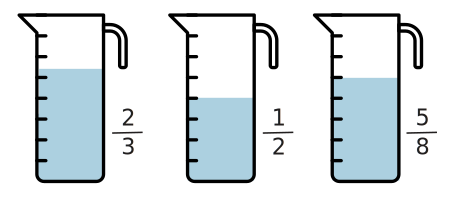
\includegraphics[width=300pt, keepaspectratio]{../../livro/media//cap4/secoes/PNGs/ativ14_fig01.png}  
\end{center}

\subsection{Atividade}

Responda às seguintes questões: 

\begin{enumerate} [\quad a)] %d
  \item     A fração determinada pela adição de 1 ao numerador da fração     $\frac{4}{7}$     é maior, menor ou igual a     $\frac{4}{7}$    ? Explique como chegou a essa conclusão.
  \item     A fração determinada pela adição de 1 ao denominador da fração     $\frac{4}{7}$     é maior, menor ou igual a     $\frac{4}{7}$    ? Explique como chegou a essa conclusão.
  \item     A fração determinada pela subtração de 1 ao denominador da fração     $\frac{4}{7}$     é maior, menor ou igual a     $\frac{4}{7}$    ? Explique como chegou a essa conclusão.
  \item     A fração determinada pela adição de 2 ao numerador e ao denominador da fração     $\frac{4}{7}$     é maior, menor ou igual a     $\frac{4}{7}$    ? Explique como chegou a essa conclusão.
  \item     A fração determinada pela multiplicação por 2 do numerador e do denominador da fração     $\frac{4}{7}$     é maior, menor ou igual a     $\frac{4}{7}$    ? Explique como chegou a essa conclusão.
  \item     A fração determinada pela adição de 1 ao numerador e subtração de 1 ao denominador da fração     $\frac{4}{7}$     é maior, menor ou igual a     $\frac{4}{7}$    ? Explique como chegou a essa conclusão.
\end{enumerate} %d

\subsection{Atividade}


(Adaptado de Empson (2001))

$24$ amigos estão querendo dividir igualmente $8$ panquecas circulares.

Luciano, um dos amigos sugeriu que cada panqueca fosse dividida em $24$ partes iguais e que, então, cada um dos 24 amigos recebesse $8$ dessas partes.
\begin{center}
 \begin{tikzpicture}[x=0.2cm,y=0.2cm, scale=1.4]
%\clip(-6.671687478832792,-17.90763699164108) rectangle (54.671411657651255,12.538800286189925);
\draw(0.,0.) circle (0.6cm);
\draw(7.,0.) circle (0.6cm);
\draw(14.,0.) circle (0.6cm);
\draw(21.,0.) circle (0.6cm);
\draw(28.,0.) circle (0.6cm);
\draw(35.,0.) circle (0.6cm);
\draw(42.,0.) circle (0.6cm);
\draw(49.,0.) circle (0.6cm);
\draw (0.,0.)-- (3.,0.);
\draw (0.,0.)-- (2.897777478867205,0.7764571353075622);
\draw (0.,0.)-- (2.598076211353316,1.5);
\draw (0.,0.)-- (2.121320343559643,2.121320343559643);
\draw (0.,0.)-- (1.5,2.5980762113533165);
\draw (0.,0.)-- (0.7764571353075628,2.8977774788672055);
\draw (0.,0.)-- (0.,3.);
\draw (0.,0.)-- (-0.776457135307562,2.8977774788672055);
\draw (0.,0.)-- (-1.5,2.5980762113533165);
\draw (0.,0.)-- (-2.121320343559643,2.1213203435596433);
\draw (0.,0.)-- (-2.5980762113533165,1.5);
\draw (0.,0.)-- (-2.897777478867206,0.7764571353075632);
\draw (0.,0.)-- (-3.,0.);
\draw (0.,0.)-- (-2.8977774788672064,-0.7764571353075619);
\draw (0.,0.)-- (-2.5980762113533173,-1.5);
\draw (0.,0.)-- (-2.121320343559644,-2.121320343559643);
\draw (0.,0.)-- (-1.5,-2.598076211353317);
\draw (0.,0.)-- (-0.7764571353075636,-2.8977774788672064);
\draw (0.,0.)-- (0.,-3.);
\draw (0.,0.)-- (0.7764571353075618,-2.8977774788672073);
\draw (0.,0.)-- (1.5,-2.5980762113533182);
\draw (0.,0.)-- (2.1213203435596433,-2.121320343559645);
\draw (0.,0.)-- (2.5980762113533173,-1.5);
\draw (0.,0.)-- (2.897777478867207,-0.7764571353075641);
\draw (4.,0.)-- (7.,0.);
\draw (4.102222521132795,0.7764571353075647)-- (7.,0.);
\draw (4.401923788646685,1.5)-- (7.,0.);
\draw (4.878679656440359,2.1213203435596446)-- (7.,0.);
\draw (5.5,2.5980762113533173)-- (7.,0.);
\draw (7.,0.)-- (6.22354286469244,2.897777478867206);
\draw (7.,0.)-- (7.,3.);
\draw (7.,0.)-- (7.776457135307564,2.8977774788672046);
\draw (7.,0.)-- (8.5,2.598076211353315);
\draw (7.,0.)-- (9.121320343559644,2.121320343559641);
\draw (7.,0.)-- (9.598076211353316,1.5);
\draw (7.,0.)-- (9.897777478867205,0.776457135307561);
\draw (7.,0.)-- (10.,0.);
\draw (7.,0.)-- (9.897777478867205,-0.7764571353075636);
\draw (7.,0.)-- (9.598076211353316,-1.5);
\draw (7.,0.)-- (9.121320343559642,-2.1213203435596433);
\draw (7.,0.)-- (8.5,-2.5980762113533165);
\draw (7.,0.)-- (7.776457135307562,-2.8977774788672055);
\draw (7.,0.)-- (7.,-3.);
\draw (7.,0.)-- (6.223542864692438,-2.8977774788672055);
\draw (7.,0.)-- (5.5,-2.5980762113533165);
\draw (7.,0.)-- (4.878679656440357,-2.121320343559643);
\draw (7.,0.)-- (4.401923788646684,-1.5);
\draw (7.,0.)-- (4.102222521132795,-0.7764571353075622);
\draw (14.,0.)-- (11.,0.);
\draw (14.,0.)-- (11.102222521132795,-0.7764571353075622);
\draw (14.,0.)-- (11.401923788646684,-1.5);
\draw (14.,0.)-- (11.878679656440358,-2.121320343559643);
\draw (14.,0.)-- (12.5,-2.598076211353316);
\draw (14.,0.)-- (13.223542864692437,-2.897777478867205);
\draw (14.,0.)-- (14.,-3.);
\draw (14.,0.)-- (14.776457135307563,-2.897777478867205);
\draw (14.,0.)-- (15.5,-2.598076211353316);
\draw (14.,0.)-- (16.121320343559642,-2.121320343559643);
\draw (14.,0.)-- (16.598076211353316,-1.5);
\draw (14.,0.)-- (16.897777478867205,-0.7764571353075631);
\draw (14.,0.)-- (17.,0.);
\draw (14.,0.)-- (16.897777478867205,0.7764571353075614);
\draw (14.,0.)-- (16.598076211353316,1.5);
\draw (14.,0.)-- (16.121320343559642,2.121320343559642);
\draw (14.,0.)-- (15.5,2.598076211353315);
\draw (14.,0.)-- (14.776457135307563,2.897777478867204);
\draw (14.,0.)-- (14.,3.);
\draw (14.,0.)-- (13.223542864692439,2.8977774788672055);
\draw (14.,0.)-- (12.5,2.598076211353317);
\draw (14.,0.)-- (11.878679656440358,2.1213203435596437);
\draw (14.,0.)-- (11.401923788646684,1.5);
\draw (14.,0.)-- (11.102222521132795,0.776457135307564);
\draw (18.,0.)-- (24.,0.);
\draw (18.102222521132795,-0.7764571353075622)-- (23.897777478867205,0.7764571353075614);
\draw (18.401923788646684,-1.5)-- (23.598076211353316,1.5);
\draw (18.878679656440358,-2.121320343559643)-- (23.121320343559642,2.121320343559642);
\draw (19.5,-2.598076211353316)-- (22.5,2.598076211353315);
\draw (20.223542864692437,-2.897777478867205)-- (21.776457135307563,2.897777478867204);
\draw (21.,-3.)-- (21.,3.);
\draw (21.776457135307563,-2.897777478867205)-- (20.223542864692437,2.897777478867205);
\draw (22.5,-2.598076211353316)-- (19.5,2.598076211353316);
\draw (23.121320343559642,-2.121320343559643)-- (18.878679656440358,2.121320343559643);
\draw (23.598076211353316,-1.5)-- (18.401923788646684,1.5);
\draw (23.897777478867205,-0.7764571353075631)-- (18.102222521132795,0.7764571353075631);
\draw (25.,0.)-- (31.,0.);
\draw (25.102222521132795,-0.7764571353075622)-- (30.897777478867205,0.7764571353075614);
\draw (25.401923788646684,-1.5)-- (30.598076211353316,1.5);
\draw (25.878679656440358,-2.121320343559643)-- (30.121320343559642,2.121320343559642);
\draw (26.5,-2.598076211353316)-- (29.5,2.598076211353315);
\draw (27.223542864692437,-2.897777478867205)-- (28.776457135307563,2.897777478867204);
\draw (28.,-3.)-- (28.,3.);
\draw (28.776457135307563,-2.897777478867205)-- (27.223542864692437,2.897777478867205);
\draw (29.5,-2.598076211353316)-- (26.5,2.598076211353316);
\draw (30.121320343559642,-2.121320343559643)-- (25.878679656440358,2.121320343559643);
\draw (30.598076211353316,-1.5)-- (25.401923788646684,1.5);
\draw (25.102222521132795,0.7764571353075631)-- (30.897777478867205,-0.7764571353075631);
\draw (32.,0.)-- (38.,0.);
\draw (32.102222521132795,-0.7764571353075622)-- (37.897777478867205,0.7764571353075614);
\draw (32.401923788646684,-1.5)-- (37.598076211353316,1.5);
\draw (32.878679656440355,-2.121320343559643)-- (37.121320343559645,2.121320343559642);
\draw (33.5,-2.598076211353317)-- (36.5,2.598076211353316);
\draw (34.22354286469244,-2.897777478867206)-- (35.77645713530756,2.897777478867205);
\draw (35.,-3.)-- (35.,3.);
\draw (35.77645713530756,-2.897777478867205)-- (34.22354286469244,2.897777478867204);
\draw (36.5,-2.598076211353317)-- (33.5,2.5980762113533165);
\draw (37.121320343559645,-2.1213203435596437)-- (32.878679656440355,2.1213203435596433);
\draw (37.598076211353316,-1.5)-- (32.401923788646684,1.5);
\draw (37.897777478867205,-0.7764571353075631)-- (32.102222521132795,0.7764571353075627);
\draw (39.,0.)-- (45.,0.);
\draw (39.102222521132795,-0.7764571353075622)-- (44.897777478867205,0.7764571353075614);
\draw (39.401923788646684,-1.5)-- (44.598076211353316,1.5);
\draw (39.878679656440355,-2.121320343559643)-- (44.121320343559645,2.121320343559642);
\draw (40.5,-2.598076211353317)-- (43.5,2.598076211353316);
\draw (41.22354286469244,-2.897777478867206)-- (42.77645713530756,2.897777478867205);
\draw (42.,-3.)-- (42.,3.);
\draw (42.77645713530756,-2.897777478867205)-- (41.22354286469244,2.897777478867204);
\draw (43.5,-2.598076211353317)-- (40.5,2.5980762113533165);
\draw (44.121320343559645,-2.1213203435596437)-- (39.878679656440355,2.1213203435596433);
\draw (44.598076211353316,-1.5)-- (39.401923788646684,1.5);
\draw (44.897777478867205,-0.7764571353075631)-- (39.102222521132795,0.7764571353075627);
\draw (46.,0.)-- (52.,0.);
\draw (46.102222521132795,-0.7764571353075622)-- (51.897777478867205,0.7764571353075614);
\draw (46.401923788646684,-1.5)-- (51.598076211353316,1.5);
\draw (46.878679656440355,-2.121320343559643)-- (51.121320343559645,2.121320343559642);
\draw (47.5,-2.598076211353317)-- (50.5,2.598076211353316);
\draw (48.22354286469244,-2.897777478867206)-- (49.77645713530756,2.897777478867205);
\draw (49.,-3.)-- (49.,3.);
\draw (49.77645713530756,-2.897777478867205)-- (48.22354286469244,2.897777478867204);
\draw (50.5,-2.598076211353317)-- (47.5,2.5980762113533165);
\draw (51.121320343559645,-2.1213203435596437)-- (46.878679656440355,2.1213203435596433);
\draw (51.598076211353316,-1.5)-- (46.401923788646684,1.5);
\draw (51.897777478867205,-0.7764571353075631)-- (46.102222521132795,0.7764571353075627);
\end{tikzpicture}
\end{center}

\begin{enumerate} [\quad a)] %d
  \item     Com a divisão sugerida por Luciano, qual a fração de uma panqueca que cada amigo vai receber?
  \item     Quantos cortes da panqueca (do centro para a borda, como no desenho) são necessários para a divisão proposta?
  \item     É possível dividir igualmente as     $8$     panquecas entre os     $24$     amigos fazendo menos cortes do que como sugerido por Luciano? Se você acha que sim, quantos cortes serão necessários e qual é a fração de uma panqueca que cada amigo vai receber neste caso?
\end{enumerate} %d

\subsection{Atividade}

Dizemos que uma fração é {\bf irredutível} se o máximo divisor comum entre o seu numerador e o seu denominador é igual a $1$. Para cada fração indicada a seguir, determine uma fração igual que seja irredutível.

\begin{tabular}{m{.18\textwidth}m{.18\textwidth}m{.18\textwidth}m{.18\textwidth}m{.18\textwidth}}
a)$\dfrac{2}{4}$, & b) $\dfrac{6}{9}$, & c) $\dfrac{4}{2}$, & d) $\dfrac{5}{35}$, & e) $\dfrac{50}{100}$. 
\end{tabular}

\subsection{Atividade}

O objetivo desta atividade é determinar qual é a maior e qual é a menor fração entre
as frações $\frac{11}{6}$, $\frac{28}{15}$ e $\frac{37}{20}$.

\begin{enumerate} [\quad a)] %s
  \item     Determine três frações de mesmo denominador que sejam iguais às frações     $\frac{11}{6}$    ,     $\frac{28}{15}$     e     $\frac{37}{20}$    .
  \item     Usando as frações do Item a), determine qual é a maior e qual é a menor fração entre as frações     $\frac{11}{6}$    ,     $\frac{28}{15}$     e     $\frac{37}{20}$    .
\end{enumerate} %s

\subsection{Atividade}

Dadas duas frações, se o produto do numerador da primeira fração pelo denominador da segunda fração for igual ao produto do denominador da primeira fração pelo numerador da segunda fração, então as frações são iguais. 

Vamos ver um exemplo: para as frações $\frac{14}{6}$ e $\frac{21}{9}$, note que  $14 \times 9 = 126 = 6 \times 21$. Vamos agora usar este fato de que $14 \times 9 = 6 \times 21$
para concluir que $\frac{14}{6} = \frac{21}{9}$:

$$\frac{14}{6} = \frac{9 \times 14}{9 \times 6} = \frac{14 \times 9}{9 \times 6} = \frac{6 \times 21}{9 \times 6} = \frac{6 \times 21}{6 \times 9} = \frac{21}{9}.$$

\begin{enumerate}[a)]
 \item Use o procedimento do exemplo para mostrar que $\frac{2}{8} = \frac{5}{20}$.
 \item Verdadeirou ou falso? Se duas frações são iguais, então o produto do numerador da primeira fração pelo denominador da segunda fração é igual ao produto do denominador da primeira fração pelo numerador da segunda fração. Justifique sua resposta.
\end{enumerate}

\subsection{Atividade}

{\bf Trilha dos doze avos}

Junte seus amigos para jogar! Seu grupo vai receber uma cópia de um tabuleiro onde há uma trilha com as posições de partida e chegada indicadas e um dado com 12 faces marcadas com os números de 1 a 12. 

\begin{center}
\begin{tikzpicture}[x=1.5cm,y=1.5cm, scale=.7]
\draw (4,0) rectangle (5,1);
\draw (3,0) rectangle (4,1);
\draw (2,0) rectangle (3,1);
\draw (1,0) rectangle (2,1);
\draw (0,0) rectangle (1,1);
\draw (0,1) rectangle (1,2);
\draw (0,2) rectangle (1,3);
\draw (0,3) rectangle (1,4);
\draw (0,4) rectangle (1,5);
\draw (0,5) rectangle (1,6);
\draw (0,6) rectangle (1,7);
\draw (0,7) rectangle (1,8);
\draw (0,8) rectangle (1,9);
\draw (0,9) rectangle (1,10);
\draw (1,9) rectangle (2,10);
\draw (2,9) rectangle (3,10);
\draw (3,9) rectangle (4,10);
\draw (4,9) rectangle (5,10);
\draw (5,9) rectangle (6,10);
\draw (6,9) rectangle (7,10);
\draw (7,9) rectangle (8,10);
\draw (8,9) rectangle (9,10);
\draw (8,8) rectangle (9,9);
\draw (8,7) rectangle (9,8);
\draw (8,6) rectangle (9,7);
\draw (8,5) rectangle (9,6);
\draw (8,4) rectangle (9,5);
\draw (8,3) rectangle (9,4);
\draw (8,2) rectangle (9,3);
\draw (7,2) rectangle (8,3);
\draw (6,2) rectangle (7,3);
\draw (5,2) rectangle (6,3);
\draw (4,2) rectangle (5,3);
\draw (3,2) rectangle (4,3);
\draw (2,2) rectangle (3,3);
\draw (2,3) rectangle (3,4);
\draw (2,4) rectangle (3,5);
\draw (2,5) rectangle (3,6);
\draw (2,6) rectangle (3,7);
\draw (2,7) rectangle (3,8);
\draw (3,7) rectangle (4,8);
\draw (4,7) rectangle (5,8);
\draw (5,7) rectangle (6,8);
\draw (6,7) rectangle (7,8);
\draw (6,6) rectangle (7,7);
\draw (6,5) rectangle (7,6);
\draw (6,4) rectangle (7,5);
\draw (5,4) rectangle (6,5);
\draw (4,4) rectangle (5,5);
\draw (4,5) rectangle (5,6);
\draw (6,0.5) node[]{PARTIDA};
\draw (4.5,6.5) node[]{CHEGADA};
\end{tikzpicture}
\end{center}

Seu grupo também receberá peões que identificarão as posições dos jogadores na trilha. Cada jogador deve escrever o seu nome no peão (na imagem a seguir, o peão está com o nome ``Antônio'').
\begin{center}
\includegraphics[width=30pt, keepaspectratio]{../../livro/media//cap4/secoes/caminho-peao.jpg}
\end{center}
O dado pode ser usado para decidir a ordem de jogada. As regras do jogo são as seguintes:


$1^{\textrm{\underline{o}}}$ No desenvolvimento do jogo, cada jogador lança o dado duas vezes. Esses lançamentos determinam a fração que correspondente ao movimento que o jogador fará: o primeiro lançamento registra o denominador da fração e o segundo o numerador. Assim, por exemplo, se o primeiro lançamento do dado resulta no número 12 e o segundo lançamento resulta no número 10, a fração correspondente é $\frac{10}{12}$. Outro exemplo: se o número do primeiro lançamento do dado é $6$ e o número do segundo lançamento é $3$, a fração correspondente é $\frac{3}{6}$. Mais um exemplo: se o número do primeiro lançamento do dado é $5$ e o número do segundo lançamento é $7$, a fração correspondente é $\frac{7}{5}$.

$2^{\textrm{\underline{o}}}$ Se a fração obtida com o lançamento dos dados for equivalente a uma fraçào de denominador 12, ou seja, a certa quantidade de doze avos, o peão ``caminha'' essa quantidade de passos. Caso contrário, ele não sai do lugar que está e passa a vez para o próximo jogador. Assim, por exemplo: se a fração obtida for $\frac{10}{12}$, seu peão andará 10 casas. Se a fração obtida for $\frac{3}{6}$, seu peão andará $6$ casas, pois $\frac{3}{6} = \frac{6}{12}$. Se a fração obtida for $\frac{7}{5}$, seu peão permanecerá na casa em que está e você passará a vez.

$3^{\textrm{\underline{o}}}$ Vence o jogo aquele jogador que, em primeiro lugar, atingir o ponto de chegada. 

Depois de jogar algumas vezes responda às questões a seguir. 


\begin{enumerate}[a)]
 \item Quantos passos um jogador deu se ele obteve nos dois lançamentos respectivamente os seguintes números:

 \noindent \begin{tabular}{m{.17\textwidth}m{.17\textwidth}m{.17\textwidth}m{.17\textwidth}m{.17\textwidth}}
1º) 12 e 7?  & 2º) 6 e 5? & 3º) 8 e 6? & 4º) 8 e 7? & 5º) 9 e 12? \\
6º) 7 e 8? & 7º) 11 e 4? & 8º) 1 e 1? & 9º) 6 e 3? & 10º) 3 e 6?
\end{tabular}

\item   Em 5 rodadas consecutivas, o primeiro jogador sorteou as frações  $\frac{7}{12}$, $\frac{10}{9}$, $\frac{1}{3}$, $\frac{3}{2}$  e  $\frac{12}{6}$. Já o segundo jogador, nessas 5 rodadas, deu ao todo 47 passos. Ao final dessas rodadas, qual deles está a frente? 
\end{enumerate}



\section{QUEBRANDO A CUCA }


\subsection{Atividade}

Jorge e Ana estão comparando as frações $\frac{2}{3}$ e $\frac{6}{10}$. Jorge afirma que 
$\frac{2}{3} < \frac{6}{10}$ porque $2 < 6$ e $3 < 10$. Ana diz que $\frac{2}{3} > \frac{6}{10}$. Use desenhos, palavras ou apenas números para ajudar Ana a explicar a Jorge porque ele está errado.

\subsection{Atividade}

Uma fração é dita {\bf unitária} se o seu numerador é igual a $1$. 
\begin{enumerate}[a)]
\item  Quais das frações a seguir são iguais a alguma fração unitária? Justifique sua resposta.

\begin{center}
\begin{tabular}{m{.13\textwidth}m{.13\textwidth}m{.13\textwidth}m{.13\textwidth}}
$\frac{4}{20}$, & $\frac{21}{7}$, & $\frac{4}{30}$, & $\frac{6}{18}$.
\end{tabular}
\end{center}

\item  Uma fração com numerador maior do que o denominador pode ser igual a uma fração unitária? Justifique sua resposta!

\item  Existe uma fração de denominador ímpar que seja igual à fração unitária $\frac{1}{2}$? Justifique sua resposta! 
\end{enumerate}

\subsection{Atividade}

Diga se cada uma das sentenças a seguir é verdadeira ou falsa. Explique a sua resposta com exemplos, desenhos ou palavras.
\begin{enumerate}[a)]
 \item  Se duas frações têm numeradores e denominadores diferentes, então elas são diferentes.
 \item Se duas frações têm denominadores iguais, mas numeradores diferentes, então elas são diferentes.
 \item Se duas frações têm numeradores iguais e maiores do que zero, mas denominadores diferentes, então elas são diferentes.
 \item Se duas frações são iguais, então o numerador e o denominador de uma são obtidos multiplicando-se o numerador e o denominador da outra por um mesmo número natural.
\end{enumerate}


\subsection{Atividade}
\begin{enumerate}[a)]
 \item Escreva uma fração que seja menor do que 1 e maior do que 0.
 \item Existe uma fração maior do que 0 e menor do que a fração que você escreveu no Item a)? Em caso afirmativo, escreva uma tal fração.
 \item Existe uma fração menor do que a fração que você escreveu no Item b)? Em caso afirmativo, escreva uma tal fração.
 \item É possível generalizar este processo, isto é, dada uma fração menor do que 1 e maior do que 0, é sempre possível determinar uma outra fração menor ainda? Em caso afirmativo, explique como tal fração pode ser obtida.
 \item Existe uma fração menor do que 1 e que seja maior do que a fração que você escreveu no Item a)? Em caso afirmativo, escreva uma tal fração.
 \item Existe uma fração menor do que 1 e que seja maior do que a fração que você escreveu no Item e)? Em caso afirmativo, escreva uma tal fração.
 \item É possível generalizar este processo, isto é, dada uma fração menor do que 1, é sempre possível determinar uma outra fração menor do que 1 e que seja maior do que a fração dada? Em caso afirmativo, explique como tal fração pode ser obtida.
\end{enumerate}

\subsection{Atividade}

Fabrício acredita que não existem frações entre $\frac{3}{5}$ e $\frac{4}{5}$ (isto é, maiores de que $\frac{3}{5}$ e menores do que $\frac{4}{5}$) porque $3 < 4$ e não existe número natural entre $3$ e $4$. Fabrício cotinua: ``Pelo mesmo motivo, não existem frações entre $\frac{11}{10}$ e $\frac{12}{10}$ e entre $\frac{19}{20}$ e $\frac{20}{20}$!''. Você concorda com as afirmações e argumentos de Fabrício? Se você acha que Fabrício está errado, determine:

\begin{enumerate}[a)]
\item  uma fração entre $\frac{3}{5}$ e $\frac{4}{5}$;

\item  duas frações entre $\frac{11}{10}$ e $\frac{12}{10}$;

\item  uma fração entre $\frac{19}{20}$ e $\frac{20}{20}$.
\end{enumerate}

\pagebreak
\begin{refletindo*}[breakable]{}{}  
  
  Nas atividades 24 e 25 você estudou uma propriedade importante do conjunto das frações:  
  
{\it  dadas quaisquer duas frações que representam diferentes quantidades, sempre é possível encontrar uma  fração entre elas.}   
  

  Ora, se sempre é possível, como se pode então determinar uma terceira fração entre as frações dadas? Para explicar melhor o procedimento, veja primeiro um exemplo.  
  
  Suponha que se quer determinar uma fração entre as frações   $\frac{5}{7}$   e   $\frac{3}{4}$  .  
  
  O primeiro passo é reescrevê-las usando um mesmo denominador:  
  
  $$\dfrac{5}{7} = \dfrac{4 \times 5}{ 4 \times 7} = \dfrac{20}{28}$$  
  e  
  $$\dfrac{3}{4} = \dfrac{7 \times 3}{ 7 \times 4} = \dfrac{21}{28}$$  
  
  Ao comparar as frações obtidas, percebe-se que   $\frac{20}{28}<\frac{21}{28}$  . No entanto, não se vê de imediato um exemplo de fração que seja maior que   $\frac{20}{28}$   e menor que   $\frac{21}{28}$  . Isto ocorre porque os números 20 e 21 são consecutivos.  
  
  Humm... que tal aumentar ainda mais os denominadores? Pois é isso que será feito.  Multiplique por dois os numeradores e denominadores de cada uma das frações. Veja:  
  
  $$\dfrac{5}{7} = \dfrac{4 \times 5}{ 4 \times 7} = \dfrac{20}{28} = \dfrac{2 \times 20}{ 2 \times 28} = \dfrac{40}{56}$$  
  e  
  $$\dfrac{3}{4} = \dfrac{7 \times 3}{ 7 \times 4} = \dfrac{21}{28} = \dfrac{2 \times 21}{2 \times 28} = \dfrac{42}{56}$$  
  
  Agora sim. Pode-se escolher a fração   $\frac{41}{56}$   como solução do problema:  
  
  $$\dfrac{5}{7} = \dfrac{4 \times 5}{ 4 \times 7} = \dfrac{20}{28} = \dfrac{2 \times 20}{ 2 \times 28} = \dfrac{40}{56} < \dfrac{41}{56} < \dfrac{42}{56} = \dfrac{2 \times 21}{2 \times 28} =  \dfrac{21}{28} = \dfrac{7 \times 3}{ 7 \times 4} = \dfrac{3}{4}.$$  
  
  De modo resumido:  
  
  $$\dfrac{5}{7} = \dfrac{40}{56} < \dfrac{41}{56} < \dfrac{42}{56} =\dfrac{3}{4}.$$  
  
  Fácil, não é mesmo? O método consiste em buscar representações equivalentes com denominadores suficientemente grandes que permitam a nossa escolha do numerador. Por isso a multiplicação simultânea dos numeradores e denominadores das frações acima por dois. Os números 20 e 21 são consecutivos, essa foi a dificuldade inicial. Mas o dobro de 20 e o dobro de 21, que são números pares, não são números consecutivos. E essa foi a jogada de mestre!  
  
  Agora sim, pode-se apresentar o procedimento utilizado em uma linguagem mais geral.  
  
  Dadas duas frações   $\frac{a}{b}$   e   $\frac{c}{d}$   diferentes (suponha   $\frac{a}{b}<\frac{c}{d}$  ) , queremos determinar uma terceira fração   $\frac{p}{q}$   tal que   $\dfrac{a}{b}<\dfrac{p}{q}<\dfrac{c}{d}$  .  
  
  O primeiro passo é encontrar frações iguais às anteriores, mas que tenham o mesmo denominador.  
  
  Para isso, basta multiplicar os numeradores e os denominadores de cada fração pelo denominador da outra fração. Veja:  
  
  $$\dfrac{a}{b} = \dfrac{d \times a}{d \times b}$$  
  onde   $d$   é o denominador da segunda fração e  
  
  $$\dfrac{c}{d} = \dfrac{b \times c}{b \times d}$$  
  onde   $b$   é o denominador da primeira fração.  
  
  Além disso, como   $\frac{a}{b}<\frac{c}{d}$  , o produto   $d \times a$   é diferente do produto   $b \times c$  .  
  
  Ora, se   $d \times a$   e   $b \times c$   não são números naturais consecutivos, já temos condições de determinar a fração   $\frac{p}{q}$   basta fazer   $q = b \times d$   e escolher um número natural   $m$   entre   $d \times a$   e   $b \times c$  . Neste caso tem-se como solução para o problema a fração  
  $$\dfrac{p}{q} = \dfrac{m}{b \times d},$$     
  onde   $m$   é um número natural entre   $d \times a$   e   $b \times c$  .  
  Agora, se   $d \times a$   e   $b \times c$   são números naturais consecutivos, usa-se a jogada de mestre. Isto é, multiplica-se por dois os numeradores e denominadores das frações acima:  
  $$\dfrac{a}{b} = \dfrac{2d \times a}{2d \times b}$$  
  e  
  $$\dfrac{c}{d} = \dfrac{2b \times c}{2b \times d}$$  
  Ora,   $(2d \times a)$    e   $(2b \times c)$   são dois números pares diferentes e, portanto, não consecutivos.   
  
  Portanto, basta escolher   $p = (2d \times a) + 1$  , o primeiro número ímpar depois do número    $(2d \times a)$  ,  e   $q=(2b \times d)$  , para encontrar uma solução do nosso problema:  
  
  $$\dfrac{a}{b} = \dfrac{2d \times a}{2d \times b} < \dfrac{(2d \times a) + 1}{2b \times d} <  \dfrac{2b \times c}{2b \times d} = \dfrac{c}{d}.$$  
  
  Isto é,   
  
  $$\dfrac{a}{b} < \dfrac{p}{q} < \dfrac{c}{d}.$$  
  
\end{refletindo*}

